\documentclass{report}

%%%%%%%%%%%%%%%%%%%%%%%%%%%%%%%%%
% PACKAGE IMPORTS
%%%%%%%%%%%%%%%%%%%%%%%%%%%%%%%%%


\usepackage[tmargin=2cm,rmargin=1in,lmargin=1in,margin=0.85in,bmargin=2cm,footskip=.2in]{geometry}
\usepackage{amsmath,amsfonts,amsthm,amssymb,mathtools}
\usepackage[varbb]{newpxmath}
\usepackage{xfrac}
\usepackage[makeroom]{cancel}
\usepackage{mathtools}
\usepackage{bookmark}
\usepackage{enumitem}
\usepackage{hyperref,theoremref}
\hypersetup{
	pdftitle={Assignment},
	colorlinks=true, linkcolor=doc!90,
	bookmarksnumbered=true,
	bookmarksopen=true
}
\usepackage[most,many,breakable]{tcolorbox}
\usepackage{xcolor}
\usepackage{varwidth}
\usepackage{varwidth}
\usepackage{etoolbox}
%\usepackage{authblk}
\usepackage{nameref}
\usepackage{multicol,array}
\usepackage{tikz-cd}
\usepackage[ruled,vlined,linesnumbered]{algorithm2e}
\usepackage{comment} % enables the use of multi-line comments (\ifx \fi) 
\usepackage{import}
\usepackage{xifthen}
\usepackage{pdfpages}
\usepackage{transparent}

\newcommand\mycommfont[1]{\footnotesize\ttfamily\textcolor{blue}{#1}}
\SetCommentSty{mycommfont}
\newcommand{\incfig}[1]{%
    \def\svgwidth{\columnwidth}
    \import{./figures/}{#1.pdf_tex}
}

\usepackage{tikzsymbols}
\renewcommand\qedsymbol{$\Laughey$}


%\usepackage{import}
%\usepackage{xifthen}
%\usepackage{pdfpages}
%\usepackage{transparent}


%%%%%%%%%%%%%%%%%%%%%%%%%%%%%%
% SELF MADE COLORS
%%%%%%%%%%%%%%%%%%%%%%%%%%%%%%



\definecolor{myg}{RGB}{56, 140, 70}
\definecolor{myb}{RGB}{45, 111, 177}
\definecolor{myr}{RGB}{199, 68, 64}
\definecolor{mytheorembg}{HTML}{F2F2F9}
\definecolor{mytheoremfr}{HTML}{00007B}
\definecolor{mylenmabg}{HTML}{FFFAF8}
\definecolor{mylenmafr}{HTML}{983b0f}
\definecolor{mypropbg}{HTML}{f2fbfc}
\definecolor{mypropfr}{HTML}{191971}
\definecolor{myexamplebg}{HTML}{F2FBF8}
\definecolor{myexamplefr}{HTML}{88D6D1}
\definecolor{myexampleti}{HTML}{2A7F7F}
\definecolor{mydefinitbg}{HTML}{E5E5FF}
\definecolor{mydefinitfr}{HTML}{3F3FA3}
\definecolor{notesgreen}{RGB}{0,162,0}
\definecolor{myp}{RGB}{197, 92, 212}
\definecolor{mygr}{HTML}{2C3338}
\definecolor{myred}{RGB}{127,0,0}
\definecolor{myyellow}{RGB}{169,121,69}
\definecolor{myexercisebg}{HTML}{F2FBF8}
\definecolor{myexercisefg}{HTML}{88D6D1}


%%%%%%%%%%%%%%%%%%%%%%%%%%%%
% TCOLORBOX SETUPS
%%%%%%%%%%%%%%%%%%%%%%%%%%%%

\setlength{\parindent}{1cm}
%================================
% THEOREM BOX
%================================

\tcbuselibrary{theorems,skins,hooks}
\newtcbtheorem[number within=section]{Theorem}{Theorem}
{%
	enhanced,
	breakable,
	colback = mytheorembg,
	frame hidden,
	boxrule = 0sp,
	borderline west = {2pt}{0pt}{mytheoremfr},
	sharp corners,
	detach title,
	before upper = \tcbtitle\par\smallskip,
	coltitle = mytheoremfr,
	fonttitle = \bfseries\sffamily,
	description font = \mdseries,
	separator sign none,
	segmentation style={solid, mytheoremfr},
}
{th}

\tcbuselibrary{theorems,skins,hooks}
\newtcbtheorem[number within=chapter]{theorem}{Theorem}
{%
	enhanced,
	breakable,
	colback = mytheorembg,
	frame hidden,
	boxrule = 0sp,
	borderline west = {2pt}{0pt}{mytheoremfr},
	sharp corners,
	detach title,
	before upper = \tcbtitle\par\smallskip,
	coltitle = mytheoremfr,
	fonttitle = \bfseries\sffamily,
	description font = \mdseries,
	separator sign none,
	segmentation style={solid, mytheoremfr},
}
{th}


\tcbuselibrary{theorems,skins,hooks}
\newtcolorbox{Theoremcon}
{%
	enhanced
	,breakable
	,colback = mytheorembg
	,frame hidden
	,boxrule = 0sp
	,borderline west = {2pt}{0pt}{mytheoremfr}
	,sharp corners
	,description font = \mdseries
	,separator sign none
}

%================================
% Corollery
%================================
\tcbuselibrary{theorems,skins,hooks}
\newtcbtheorem[number within=section]{Corollary}{Corollary}
{%
	enhanced
	,breakable
	,colback = myp!10
	,frame hidden
	,boxrule = 0sp
	,borderline west = {2pt}{0pt}{myp!85!black}
	,sharp corners
	,detach title
	,before upper = \tcbtitle\par\smallskip
	,coltitle = myp!85!black
	,fonttitle = \bfseries\sffamily
	,description font = \mdseries
	,separator sign none
	,segmentation style={solid, myp!85!black}
}
{th}
\tcbuselibrary{theorems,skins,hooks}
\newtcbtheorem[number within=chapter]{corollary}{Corollary}
{%
	enhanced
	,breakable
	,colback = myp!10
	,frame hidden
	,boxrule = 0sp
	,borderline west = {2pt}{0pt}{myp!85!black}
	,sharp corners
	,detach title
	,before upper = \tcbtitle\par\smallskip
	,coltitle = myp!85!black
	,fonttitle = \bfseries\sffamily
	,description font = \mdseries
	,separator sign none
	,segmentation style={solid, myp!85!black}
}
{th}


%================================
% LENMA
%================================

\tcbuselibrary{theorems,skins,hooks}
\newtcbtheorem[number within=section]{Lenma}{Lenma}
{%
	enhanced,
	breakable,
	colback = mylenmabg,
	frame hidden,
	boxrule = 0sp,
	borderline west = {2pt}{0pt}{mylenmafr},
	sharp corners,
	detach title,
	before upper = \tcbtitle\par\smallskip,
	coltitle = mylenmafr,
	fonttitle = \bfseries\sffamily,
	description font = \mdseries,
	separator sign none,
	segmentation style={solid, mylenmafr},
}
{th}

\tcbuselibrary{theorems,skins,hooks}
\newtcbtheorem[number within=chapter]{lenma}{Lenma}
{%
	enhanced,
	breakable,
	colback = mylenmabg,
	frame hidden,
	boxrule = 0sp,
	borderline west = {2pt}{0pt}{mylenmafr},
	sharp corners,
	detach title,
	before upper = \tcbtitle\par\smallskip,
	coltitle = mylenmafr,
	fonttitle = \bfseries\sffamily,
	description font = \mdseries,
	separator sign none,
	segmentation style={solid, mylenmafr},
}
{th}


%================================
% PROPOSITION
%================================

\tcbuselibrary{theorems,skins,hooks}
\newtcbtheorem[number within=section]{Prop}{Proposition}
{%
	enhanced,
	breakable,
	colback = mypropbg,
	frame hidden,
	boxrule = 0sp,
	borderline west = {2pt}{0pt}{mypropfr},
	sharp corners,
	detach title,
	before upper = \tcbtitle\par\smallskip,
	coltitle = mypropfr,
	fonttitle = \bfseries\sffamily,
	description font = \mdseries,
	separator sign none,
	segmentation style={solid, mypropfr},
}
{th}

\tcbuselibrary{theorems,skins,hooks}
\newtcbtheorem[number within=chapter]{prop}{Proposition}
{%
	enhanced,
	breakable,
	colback = mypropbg,
	frame hidden,
	boxrule = 0sp,
	borderline west = {2pt}{0pt}{mypropfr},
	sharp corners,
	detach title,
	before upper = \tcbtitle\par\smallskip,
	coltitle = mypropfr,
	fonttitle = \bfseries\sffamily,
	description font = \mdseries,
	separator sign none,
	segmentation style={solid, mypropfr},
}
{th}


%================================
% CLAIM
%================================

\tcbuselibrary{theorems,skins,hooks}
\newtcbtheorem[number within=section]{claim}{Claim}
{%
	enhanced
	,breakable
	,colback = myg!10
	,frame hidden
	,boxrule = 0sp
	,borderline west = {2pt}{0pt}{myg}
	,sharp corners
	,detach title
	,before upper = \tcbtitle\par\smallskip
	,coltitle = myg!85!black
	,fonttitle = \bfseries\sffamily
	,description font = \mdseries
	,separator sign none
	,segmentation style={solid, myg!85!black}
}
{th}



%================================
% Exercise
%================================

\tcbuselibrary{theorems,skins,hooks}
\newtcbtheorem[number within=section]{Exercise}{Exercise}
{%
	enhanced,
	breakable,
	colback = myexercisebg,
	frame hidden,
	boxrule = 0sp,
	borderline west = {2pt}{0pt}{myexercisefg},
	sharp corners,
	detach title,
	before upper = \tcbtitle\par\smallskip,
	coltitle = myexercisefg,
	fonttitle = \bfseries\sffamily,
	description font = \mdseries,
	separator sign none,
	segmentation style={solid, myexercisefg},
}
{th}

\tcbuselibrary{theorems,skins,hooks}
\newtcbtheorem[number within=chapter]{exercise}{Exercise}
{%
	enhanced,
	breakable,
	colback = myexercisebg,
	frame hidden,
	boxrule = 0sp,
	borderline west = {2pt}{0pt}{myexercisefg},
	sharp corners,
	detach title,
	before upper = \tcbtitle\par\smallskip,
	coltitle = myexercisefg,
	fonttitle = \bfseries\sffamily,
	description font = \mdseries,
	separator sign none,
	segmentation style={solid, myexercisefg},
}
{th}

%================================
% EXAMPLE BOX
%================================

\newtcbtheorem[number within=section]{Example}{Example}
{%
	colback = myexamplebg
	,breakable
	,colframe = myexamplefr
	,coltitle = myexampleti
	,boxrule = 1pt
	,sharp corners
	,detach title
	,before upper=\tcbtitle\par\smallskip
	,fonttitle = \bfseries
	,description font = \mdseries
	,separator sign none
	,description delimiters parenthesis
}
{ex}

\newtcbtheorem[number within=chapter]{example}{Example}
{%
	colback = myexamplebg
	,breakable
	,colframe = myexamplefr
	,coltitle = myexampleti
	,boxrule = 1pt
	,sharp corners
	,detach title
	,before upper=\tcbtitle\par\smallskip
	,fonttitle = \bfseries
	,description font = \mdseries
	,separator sign none
	,description delimiters parenthesis
}
{ex}

%================================
% DEFINITION BOX
%================================

\newtcbtheorem[number within=section]{Definition}{Definition}{enhanced,
	before skip=2mm,after skip=2mm, colback=red!5,colframe=red!80!black,boxrule=0.5mm,
	attach boxed title to top left={xshift=1cm,yshift*=1mm-\tcboxedtitleheight}, varwidth boxed title*=-3cm,
	boxed title style={frame code={
					\path[fill=tcbcolback]
					([yshift=-1mm,xshift=-1mm]frame.north west)
					arc[start angle=0,end angle=180,radius=1mm]
					([yshift=-1mm,xshift=1mm]frame.north east)
					arc[start angle=180,end angle=0,radius=1mm];
					\path[left color=tcbcolback!60!black,right color=tcbcolback!60!black,
						middle color=tcbcolback!80!black]
					([xshift=-2mm]frame.north west) -- ([xshift=2mm]frame.north east)
					[rounded corners=1mm]-- ([xshift=1mm,yshift=-1mm]frame.north east)
					-- (frame.south east) -- (frame.south west)
					-- ([xshift=-1mm,yshift=-1mm]frame.north west)
					[sharp corners]-- cycle;
				},interior engine=empty,
		},
	fonttitle=\bfseries,
	title={#2},#1}{def}
\newtcbtheorem[number within=chapter]{definition}{Definition}{enhanced,
	before skip=2mm,after skip=2mm, colback=red!5,colframe=red!80!black,boxrule=0.5mm,
	attach boxed title to top left={xshift=1cm,yshift*=1mm-\tcboxedtitleheight}, varwidth boxed title*=-3cm,
	boxed title style={frame code={
					\path[fill=tcbcolback]
					([yshift=-1mm,xshift=-1mm]frame.north west)
					arc[start angle=0,end angle=180,radius=1mm]
					([yshift=-1mm,xshift=1mm]frame.north east)
					arc[start angle=180,end angle=0,radius=1mm];
					\path[left color=tcbcolback!60!black,right color=tcbcolback!60!black,
						middle color=tcbcolback!80!black]
					([xshift=-2mm]frame.north west) -- ([xshift=2mm]frame.north east)
					[rounded corners=1mm]-- ([xshift=1mm,yshift=-1mm]frame.north east)
					-- (frame.south east) -- (frame.south west)
					-- ([xshift=-1mm,yshift=-1mm]frame.north west)
					[sharp corners]-- cycle;
				},interior engine=empty,
		},
	fonttitle=\bfseries,
	title={#2},#1}{def}



%================================
% Solution BOX
%================================

\makeatletter
\newtcbtheorem{question}{Question}{enhanced,
	breakable,
	colback=white,
	colframe=myb!80!black,
	attach boxed title to top left={yshift*=-\tcboxedtitleheight},
	fonttitle=\bfseries,
	title={#2},
	boxed title size=title,
	boxed title style={%
			sharp corners,
			rounded corners=northwest,
			colback=tcbcolframe,
			boxrule=0pt,
		},
	underlay boxed title={%
			\path[fill=tcbcolframe] (title.south west)--(title.south east)
			to[out=0, in=180] ([xshift=5mm]title.east)--
			(title.center-|frame.east)
			[rounded corners=\kvtcb@arc] |-
			(frame.north) -| cycle;
		},
	#1
}{def}
\makeatother

%================================
% SOLUTION BOX
%================================

\makeatletter
\newtcolorbox{solution}{enhanced,
	breakable,
	colback=white,
	colframe=myg!80!black,
	attach boxed title to top left={yshift*=-\tcboxedtitleheight},
	title=Solution,
	boxed title size=title,
	boxed title style={%
			sharp corners,
			rounded corners=northwest,
			colback=tcbcolframe,
			boxrule=0pt,
		},
	underlay boxed title={%
			\path[fill=tcbcolframe] (title.south west)--(title.south east)
			to[out=0, in=180] ([xshift=5mm]title.east)--
			(title.center-|frame.east)
			[rounded corners=\kvtcb@arc] |-
			(frame.north) -| cycle;
		},
}
\makeatother

%================================
% Question BOX
%================================

\makeatletter
\newtcbtheorem{qstion}{Question}{enhanced,
	breakable,
	colback=white,
	colframe=mygr,
	attach boxed title to top left={yshift*=-\tcboxedtitleheight},
	fonttitle=\bfseries,
	title={#2},
	boxed title size=title,
	boxed title style={%
			sharp corners,
			rounded corners=northwest,
			colback=tcbcolframe,
			boxrule=0pt,
		},
	underlay boxed title={%
			\path[fill=tcbcolframe] (title.south west)--(title.south east)
			to[out=0, in=180] ([xshift=5mm]title.east)--
			(title.center-|frame.east)
			[rounded corners=\kvtcb@arc] |-
			(frame.north) -| cycle;
		},
	#1
}{def}
\makeatother

\newtcbtheorem[number within=chapter]{wconc}{Wrong Concept}{
	breakable,
	enhanced,
	colback=white,
	colframe=myr,
	arc=0pt,
	outer arc=0pt,
	fonttitle=\bfseries\sffamily\large,
	colbacktitle=myr,
	attach boxed title to top left={},
	boxed title style={
			enhanced,
			skin=enhancedfirst jigsaw,
			arc=3pt,
			bottom=0pt,
			interior style={fill=myr}
		},
	#1
}{def}



%================================
% NOTE BOX
%================================

\usetikzlibrary{arrows,calc,shadows.blur}
\tcbuselibrary{skins}
\newtcolorbox{note}[1][]{%
	enhanced jigsaw,
	colback=gray!20!white,%
	colframe=gray!80!black,
	size=small,
	boxrule=1pt,
	title=\textbf{Note:-},
	halign title=flush center,
	coltitle=black,
	breakable,
	drop shadow=black!50!white,
	attach boxed title to top left={xshift=1cm,yshift=-\tcboxedtitleheight/2,yshifttext=-\tcboxedtitleheight/2},
	minipage boxed title=1.5cm,
	boxed title style={%
			colback=white,
			size=fbox,
			boxrule=1pt,
			boxsep=2pt,
			underlay={%
					\coordinate (dotA) at ($(interior.west) + (-0.5pt,0)$);
					\coordinate (dotB) at ($(interior.east) + (0.5pt,0)$);
					\begin{scope}
						\clip (interior.north west) rectangle ([xshift=3ex]interior.east);
						\filldraw [white, blur shadow={shadow opacity=60, shadow yshift=-.75ex}, rounded corners=2pt] (interior.north west) rectangle (interior.south east);
					\end{scope}
					\begin{scope}[gray!80!black]
						\fill (dotA) circle (2pt);
						\fill (dotB) circle (2pt);
					\end{scope}
				},
		},
	#1,
}

%%%%%%%%%%%%%%%%%%%%%%%%%%%%%%
% SELF MADE COMMANDS
%%%%%%%%%%%%%%%%%%%%%%%%%%%%%%


\newcommand{\thm}[2]{\begin{Theorem}{#1}{}#2\end{Theorem}}
\newcommand{\cor}[2]{\begin{Corollary}{#1}{}#2\end{Corollary}}
\newcommand{\mlenma}[2]{\begin{Lenma}{#1}{}#2\end{Lenma}}
\newcommand{\mprop}[2]{\begin{Prop}{#1}{}#2\end{Prop}}
\newcommand{\clm}[3]{\begin{claim}{#1}{#2}#3\end{claim}}
\newcommand{\wc}[2]{\begin{wconc}{#1}{}\setlength{\parindent}{1cm}#2\end{wconc}}
\newcommand{\thmcon}[1]{\begin{Theoremcon}{#1}\end{Theoremcon}}
\newcommand{\ex}[2]{\begin{Example}{#1}{}#2\end{Example}}
\newcommand{\dfn}[2]{\begin{Definition}[colbacktitle=red!75!black]{#1}{}#2\end{Definition}}
\newcommand{\dfnc}[2]{\begin{definition}[colbacktitle=red!75!black]{#1}{}#2\end{definition}}
\newcommand{\qs}[2]{\begin{question}{#1}{}#2\end{question}}
\newcommand{\pf}[2]{\begin{myproof}[#1]#2\end{myproof}}
\newcommand{\nt}[1]{\begin{note}#1\end{note}}
\newcommand{\mat}[1]{\begin{bmatrix} #1 \end{bmatrix}}
\newcommand{\vect}[1]{\begin{bmatrix} #1 \end{bmatrix}}

\newcommand*\circled[1]{\tikz[baseline=(char.base)]{
		\node[shape=circle,draw,inner sep=1pt] (char) {#1};}}
\newcommand\getcurrentref[1]{%
	\ifnumequal{\value{#1}}{0}
	{??}
	{\the\value{#1}}%
}
\newcommand{\getCurrentSectionNumber}{\getcurrentref{section}}
\newenvironment{myproof}[1][\proofname]{%
	\proof[\bfseries #1: ]%
}{\endproof}

\newcommand{\mclm}[2]{\begin{myclaim}[#1]#2\end{myclaim}}
\newenvironment{myclaim}[1][\claimname]{\proof[\bfseries #1: ]}{}

\newcounter{mylabelcounter}

\makeatletter
\newcommand{\setword}[2]{%
	\phantomsection
	#1\def\@currentlabel{\unexpanded{#1}}\label{#2}%
}
\makeatother




\tikzset{
	symbol/.style={
			draw=none,
			every to/.append style={
					edge node={node [sloped, allow upside down, auto=false]{$#1$}}}
		}
}


% deliminators
\DeclarePairedDelimiter{\abs}{\lvert}{\rvert}
\DeclarePairedDelimiter{\norm}{\lVert}{\rVert}

\DeclarePairedDelimiter{\ceil}{\lceil}{\rceil}
\DeclarePairedDelimiter{\floor}{\lfloor}{\rfloor}
\DeclarePairedDelimiter{\round}{\lfloor}{\rceil}

\newsavebox\diffdbox
\newcommand{\slantedromand}{{\mathpalette\makesl{d}}}
\newcommand{\makesl}[2]{%
\begingroup
\sbox{\diffdbox}{$\mathsurround=0pt#1\mathrm{#2}$}%
\pdfsave
\pdfsetmatrix{1 0 0.2 1}%
\rlap{\usebox{\diffdbox}}%
\pdfrestore
\hskip\wd\diffdbox
\endgroup
}
\newcommand{\dd}[1][]{\ensuremath{\mathop{}\!\ifstrempty{#1}{%
\slantedromand\@ifnextchar^{\hspace{0.2ex}}{\hspace{0.1ex}}}%
{\slantedromand\hspace{0.2ex}^{#1}}}}
\ProvideDocumentCommand\dv{o m g}{%
  \ensuremath{%
    \IfValueTF{#3}{%
      \IfNoValueTF{#1}{%
        \frac{\dd #2}{\dd #3}%
      }{%
        \frac{\dd^{#1} #2}{\dd #3^{#1}}%
      }%
    }{%
      \IfNoValueTF{#1}{%
        \frac{\dd}{\dd #2}%
      }{%
        \frac{\dd^{#1}}{\dd #2^{#1}}%
      }%
    }%
  }%
}
\providecommand*{\pdv}[3][]{\frac{\partial^{#1}#2}{\partial#3^{#1}}}
%  - others
\DeclareMathOperator{\Lap}{\mathcal{L}}
\DeclareMathOperator{\Var}{Var} % varience
\DeclareMathOperator{\Cov}{Cov} % covarience
\DeclareMathOperator{\E}{E} % expected

% Since the amsthm package isn't loaded

% I prefer the slanted \leq
\let\oldleq\leq % save them in case they're every wanted
\let\oldgeq\geq
\renewcommand{\leq}{\leqslant}
\renewcommand{\geq}{\geqslant}

% % redefine matrix env to allow for alignment, use r as default
% \renewcommand*\env@matrix[1][r]{\hskip -\arraycolsep
%     \let\@ifnextchar\new@ifnextchar
%     \array{*\c@MaxMatrixCols #1}}


%\usepackage{framed}
%\usepackage{titletoc}
%\usepackage{etoolbox}
%\usepackage{lmodern}


%\patchcmd{\tableofcontents}{\contentsname}{\sffamily\contentsname}{}{}

%\renewenvironment{leftbar}
%{\def\FrameCommand{\hspace{6em}%
%		{\color{myyellow}\vrule width 2pt depth 6pt}\hspace{1em}}%
%	\MakeFramed{\parshape 1 0cm \dimexpr\textwidth-6em\relax\FrameRestore}\vskip2pt%
%}
%{\endMakeFramed}

%\titlecontents{chapter}
%[0em]{\vspace*{2\baselineskip}}
%{\parbox{4.5em}{%
%		\hfill\Huge\sffamily\bfseries\color{myred}\thecontentspage}%
%	\vspace*{-2.3\baselineskip}\leftbar\textsc{\small\chaptername~\thecontentslabel}\\\sffamily}
%{}{\endleftbar}
%\titlecontents{section}
%[8.4em]
%{\sffamily\contentslabel{3em}}{}{}
%{\hspace{0.5em}\nobreak\itshape\color{myred}\contentspage}
%\titlecontents{subsection}
%[8.4em]
%{\sffamily\contentslabel{3em}}{}{}  
%{\hspace{0.5em}\nobreak\itshape\color{myred}\contentspage}



%%%%%%%%%%%%%%%%%%%%%%%%%%%%%%%%%%%%%%%%%%%
% TABLE OF CONTENTS
%%%%%%%%%%%%%%%%%%%%%%%%%%%%%%%%%%%%%%%%%%%

\usepackage{tikz}
\definecolor{doc}{RGB}{0,60,110}
\usepackage{titletoc}
\contentsmargin{0cm}
\titlecontents{chapter}[3.7pc]
{\addvspace{30pt}%
	\begin{tikzpicture}[remember picture, overlay]%
		\draw[fill=doc!60,draw=doc!60] (-7,-.1) rectangle (-0.9,.5);%
		\pgftext[left,x=-3.5cm,y=0.2cm]{\color{white}\Large\sc\bfseries Chapter\ \thecontentslabel};%
	\end{tikzpicture}\color{doc!60}\large\sc\bfseries}%
{}
{}
{\;\titlerule\;\large\sc\bfseries Page \thecontentspage
	\begin{tikzpicture}[remember picture, overlay]
		\draw[fill=doc!60,draw=doc!60] (2pt,0) rectangle (4,0.1pt);
	\end{tikzpicture}}%
\titlecontents{section}[3.7pc]
{\addvspace{2pt}}
{\contentslabel[\thecontentslabel]{2pc}}
{}
{\hfill\small \thecontentspage}
[]
\titlecontents*{subsection}[3.7pc]
{\addvspace{-1pt}\small}
{}
{}
{\ --- \small\thecontentspage}
[ \textbullet\ ][]

\makeatletter
\renewcommand{\tableofcontents}{%
	\chapter*{%
	  \vspace*{-20\p@}%
	  \begin{tikzpicture}[remember picture, overlay]%
		  \pgftext[right,x=15cm,y=0.2cm]{\color{doc!60}\Huge\sc\bfseries \contentsname};%
		  \draw[fill=doc!60,draw=doc!60] (13,-.75) rectangle (20,1);%
		  \clip (13,-.75) rectangle (20,1);
		  \pgftext[right,x=15cm,y=0.2cm]{\color{white}\Huge\sc\bfseries \contentsname};%
	  \end{tikzpicture}}%
	\@starttoc{toc}}
\makeatother


%From M275 "Topology" at SJSU
\newcommand{\id}{\mathrm{id}}
\newcommand{\taking}[1]{\xrightarrow{#1}}
\newcommand{\inv}{^{-1}}

%From M170 "Introduction to Graph Theory" at SJSU
\DeclareMathOperator{\diam}{diam}
\DeclareMathOperator{\ord}{ord}
\newcommand{\defeq}{\overset{\mathrm{def}}{=}}

%From the USAMO .tex files
\newcommand{\ts}{\textsuperscript}
\newcommand{\dg}{^\circ}
\newcommand{\ii}{\item}

% % From Math 55 and Math 145 at Harvard
% \newenvironment{subproof}[1][Proof]{%
% \begin{proof}[#1] \renewcommand{\qedsymbol}{$\blacksquare$}}%
% {\end{proof}}

\newcommand{\liff}{\leftrightarrow}
\newcommand{\lthen}{\rightarrow}
\newcommand{\opname}{\operatorname}
\newcommand{\surjto}{\twoheadrightarrow}
\newcommand{\injto}{\hookrightarrow}
\newcommand{\On}{\mathrm{On}} % ordinals
\DeclareMathOperator{\img}{im} % Image
\DeclareMathOperator{\Img}{Im} % Image
\DeclareMathOperator{\coker}{coker} % Cokernel
\DeclareMathOperator{\Coker}{Coker} % Cokernel
\DeclareMathOperator{\Ker}{Ker} % Kernel
\DeclareMathOperator{\rank}{rank}
\DeclareMathOperator{\Spec}{Spec} % spectrum
\DeclareMathOperator{\Tr}{Tr} % trace
\DeclareMathOperator{\pr}{pr} % projection
\DeclareMathOperator{\ext}{ext} % extension
\DeclareMathOperator{\pred}{pred} % predecessor
\DeclareMathOperator{\dom}{dom} % domain
\DeclareMathOperator{\ran}{ran} % range
\DeclareMathOperator{\Hom}{Hom} % homomorphism
\DeclareMathOperator{\Mor}{Mor} % morphisms
\DeclareMathOperator{\End}{End} % endomorphism

\newcommand{\eps}{\epsilon}
\newcommand{\veps}{\varepsilon}
\newcommand{\ol}{\overline}
\newcommand{\ul}{\underline}
\newcommand{\wt}{\widetilde}
\newcommand{\wh}{\widehat}
\newcommand{\vocab}[1]{\textbf{\color{blue} #1}}
\providecommand{\half}{\frac{1}{2}}
\newcommand{\dang}{\measuredangle} %% Directed angle
\newcommand{\ray}[1]{\overrightarrow{#1}}
\newcommand{\seg}[1]{\overline{#1}}
\newcommand{\arc}[1]{\wideparen{#1}}
\DeclareMathOperator{\cis}{cis}
\DeclareMathOperator*{\lcm}{lcm}
\DeclareMathOperator*{\argmin}{arg min}
\DeclareMathOperator*{\argmax}{arg max}
\newcommand{\cycsum}{\sum_{\mathrm{cyc}}}
\newcommand{\symsum}{\sum_{\mathrm{sym}}}
\newcommand{\cycprod}{\prod_{\mathrm{cyc}}}
\newcommand{\symprod}{\prod_{\mathrm{sym}}}
\newcommand{\Qed}{\begin{flushright}\qed\end{flushright}}
\newcommand{\parinn}{\setlength{\parindent}{1cm}}
\newcommand{\parinf}{\setlength{\parindent}{0cm}}
% \newcommand{\norm}{\|\cdot\|}
\newcommand{\inorm}{\norm_{\infty}}
\newcommand{\opensets}{\{V_{\alpha}\}_{\alpha\in I}}
\newcommand{\oset}{V_{\alpha}}
\newcommand{\opset}[1]{V_{\alpha_{#1}}}
\newcommand{\lub}{\text{lub}}
\newcommand{\del}[2]{\frac{\partial #1}{\partial #2}}
\newcommand{\Del}[3]{\frac{\partial^{#1} #2}{\partial^{#1} #3}}
\newcommand{\deld}[2]{\dfrac{\partial #1}{\partial #2}}
\newcommand{\Deld}[3]{\dfrac{\partial^{#1} #2}{\partial^{#1} #3}}
\newcommand{\lm}{\lambda}
\newcommand{\uin}{\mathbin{\rotatebox[origin=c]{90}{$\in$}}}
\newcommand{\usubset}{\mathbin{\rotatebox[origin=c]{90}{$\subset$}}}
\newcommand{\lt}{\left}
\newcommand{\rt}{\right}
\newcommand{\bs}[1]{\boldsymbol{#1}}
\newcommand{\exs}{\exists}
\newcommand{\st}{\strut}
\newcommand{\dps}[1]{\displaystyle{#1}}

\newcommand{\sol}{\setlength{\parindent}{0cm}\textbf{\textit{Solution:}}\setlength{\parindent}{1cm} }
\newcommand{\solve}[1]{\setlength{\parindent}{0cm}\textbf{\textit{Solution: }}\setlength{\parindent}{1cm}#1 \Qed}

% Things Lie
\newcommand{\kb}{\mathfrak b}
\newcommand{\kg}{\mathfrak g}
\newcommand{\kh}{\mathfrak h}
\newcommand{\kn}{\mathfrak n}
\newcommand{\ku}{\mathfrak u}
\newcommand{\kz}{\mathfrak z}
\DeclareMathOperator{\Ext}{Ext} % Ext functor
\DeclareMathOperator{\Tor}{Tor} % Tor functor
\newcommand{\gl}{\opname{\mathfrak{gl}}} % frak gl group
\renewcommand{\sl}{\opname{\mathfrak{sl}}} % frak sl group chktex 6

% More script letters etc.
\newcommand{\SA}{\mathcal A}
\newcommand{\SB}{\mathcal B}
\newcommand{\SC}{\mathcal C}
\newcommand{\SF}{\mathcal F}
\newcommand{\SG}{\mathcal G}
\newcommand{\SH}{\mathcal H}
\newcommand{\OO}{\mathcal O}

\newcommand{\SCA}{\mathscr A}
\newcommand{\SCB}{\mathscr B}
\newcommand{\SCC}{\mathscr C}
\newcommand{\SCD}{\mathscr D}
\newcommand{\SCE}{\mathscr E}
\newcommand{\SCF}{\mathscr F}
\newcommand{\SCG}{\mathscr G}
\newcommand{\SCH}{\mathscr H}

% Mathfrak primes
\newcommand{\km}{\mathfrak m}
\newcommand{\kp}{\mathfrak p}
\newcommand{\kq}{\mathfrak q}

% number sets
\newcommand{\RR}[1][]{\ensuremath{\ifstrempty{#1}{\mathbb{R}}{\mathbb{R}^{#1}}}}
\newcommand{\NN}[1][]{\ensuremath{\ifstrempty{#1}{\mathbb{N}}{\mathbb{N}^{#1}}}}
\newcommand{\ZZ}[1][]{\ensuremath{\ifstrempty{#1}{\mathbb{Z}}{\mathbb{Z}^{#1}}}}
\newcommand{\QQ}[1][]{\ensuremath{\ifstrempty{#1}{\mathbb{Q}}{\mathbb{Q}^{#1}}}}
\newcommand{\CC}[1][]{\ensuremath{\ifstrempty{#1}{\mathbb{C}}{\mathbb{C}^{#1}}}}
\newcommand{\PP}[1][]{\ensuremath{\ifstrempty{#1}{\mathbb{P}}{\mathbb{P}^{#1}}}}
\newcommand{\HH}[1][]{\ensuremath{\ifstrempty{#1}{\mathbb{H}}{\mathbb{H}^{#1}}}}
\newcommand{\FF}[1][]{\ensuremath{\ifstrempty{#1}{\mathbb{F}}{\mathbb{F}^{#1}}}}
% expected value
\newcommand{\EE}{\ensuremath{\mathbb{E}}}
\newcommand{\charin}{\text{ char }}
\DeclareMathOperator{\sign}{sign}
\DeclareMathOperator{\Aut}{Aut}
\DeclareMathOperator{\Inn}{Inn}
\DeclareMathOperator{\Syl}{Syl}
\DeclareMathOperator{\Gal}{Gal}
\DeclareMathOperator{\GL}{GL} % General linear group
\DeclareMathOperator{\SL}{SL} % Special linear group

%---------------------------------------
% BlackBoard Math Fonts :-
%---------------------------------------

%Captital Letters
\newcommand{\bbA}{\mathbb{A}}	\newcommand{\bbB}{\mathbb{B}}
\newcommand{\bbC}{\mathbb{C}}	\newcommand{\bbD}{\mathbb{D}}
\newcommand{\bbE}{\mathbb{E}}	\newcommand{\bbF}{\mathbb{F}}
\newcommand{\bbG}{\mathbb{G}}	\newcommand{\bbH}{\mathbb{H}}
\newcommand{\bbI}{\mathbb{I}}	\newcommand{\bbJ}{\mathbb{J}}
\newcommand{\bbK}{\mathbb{K}}	\newcommand{\bbL}{\mathbb{L}}
\newcommand{\bbM}{\mathbb{M}}	\newcommand{\bbN}{\mathbb{N}}
\newcommand{\bbO}{\mathbb{O}}	\newcommand{\bbP}{\mathbb{P}}
\newcommand{\bbQ}{\mathbb{Q}}	\newcommand{\bbR}{\mathbb{R}}
\newcommand{\bbS}{\mathbb{S}}	\newcommand{\bbT}{\mathbb{T}}
\newcommand{\bbU}{\mathbb{U}}	\newcommand{\bbV}{\mathbb{V}}
\newcommand{\bbW}{\mathbb{W}}	\newcommand{\bbX}{\mathbb{X}}
\newcommand{\bbY}{\mathbb{Y}}	\newcommand{\bbZ}{\mathbb{Z}}

%---------------------------------------
% MathCal Fonts :-
%---------------------------------------

%Captital Letters
\newcommand{\mcA}{\mathcal{A}}	\newcommand{\mcB}{\mathcal{B}}
\newcommand{\mcC}{\mathcal{C}}	\newcommand{\mcD}{\mathcal{D}}
\newcommand{\mcE}{\mathcal{E}}	\newcommand{\mcF}{\mathcal{F}}
\newcommand{\mcG}{\mathcal{G}}	\newcommand{\mcH}{\mathcal{H}}
\newcommand{\mcI}{\mathcal{I}}	\newcommand{\mcJ}{\mathcal{J}}
\newcommand{\mcK}{\mathcal{K}}	\newcommand{\mcL}{\mathcal{L}}
\newcommand{\mcM}{\mathcal{M}}	\newcommand{\mcN}{\mathcal{N}}
\newcommand{\mcO}{\mathcal{O}}	\newcommand{\mcP}{\mathcal{P}}
\newcommand{\mcQ}{\mathcal{Q}}	\newcommand{\mcR}{\mathcal{R}}
\newcommand{\mcS}{\mathcal{S}}	\newcommand{\mcT}{\mathcal{T}}
\newcommand{\mcU}{\mathcal{U}}	\newcommand{\mcV}{\mathcal{V}}
\newcommand{\mcW}{\mathcal{W}}	\newcommand{\mcX}{\mathcal{X}}
\newcommand{\mcY}{\mathcal{Y}}	\newcommand{\mcZ}{\mathcal{Z}}


%---------------------------------------
% Bold Math Fonts :-
%---------------------------------------

%Captital Letters
\newcommand{\bmA}{\boldsymbol{A}}	\newcommand{\bmB}{\boldsymbol{B}}
\newcommand{\bmC}{\boldsymbol{C}}	\newcommand{\bmD}{\boldsymbol{D}}
\newcommand{\bmE}{\boldsymbol{E}}	\newcommand{\bmF}{\boldsymbol{F}}
\newcommand{\bmG}{\boldsymbol{G}}	\newcommand{\bmH}{\boldsymbol{H}}
\newcommand{\bmI}{\boldsymbol{I}}	\newcommand{\bmJ}{\boldsymbol{J}}
\newcommand{\bmK}{\boldsymbol{K}}	\newcommand{\bmL}{\boldsymbol{L}}
\newcommand{\bmM}{\boldsymbol{M}}	\newcommand{\bmN}{\boldsymbol{N}}
\newcommand{\bmO}{\boldsymbol{O}}	\newcommand{\bmP}{\boldsymbol{P}}
\newcommand{\bmQ}{\boldsymbol{Q}}	\newcommand{\bmR}{\boldsymbol{R}}
\newcommand{\bmS}{\boldsymbol{S}}	\newcommand{\bmT}{\boldsymbol{T}}
\newcommand{\bmU}{\boldsymbol{U}}	\newcommand{\bmV}{\boldsymbol{V}}
\newcommand{\bmW}{\boldsymbol{W}}	\newcommand{\bmX}{\boldsymbol{X}}
\newcommand{\bmY}{\boldsymbol{Y}}	\newcommand{\bmZ}{\boldsymbol{Z}}
%Small Letters
\newcommand{\bma}{\boldsymbol{a}}	\newcommand{\bmb}{\boldsymbol{b}}
\newcommand{\bmc}{\boldsymbol{c}}	\newcommand{\bmd}{\boldsymbol{d}}
\newcommand{\bme}{\boldsymbol{e}}	\newcommand{\bmf}{\boldsymbol{f}}
\newcommand{\bmg}{\boldsymbol{g}}	\newcommand{\bmh}{\boldsymbol{h}}
\newcommand{\bmi}{\boldsymbol{i}}	\newcommand{\bmj}{\boldsymbol{j}}
\newcommand{\bmk}{\boldsymbol{k}}	\newcommand{\bml}{\boldsymbol{l}}
\newcommand{\bmm}{\boldsymbol{m}}	\newcommand{\bmn}{\boldsymbol{n}}
\newcommand{\bmo}{\boldsymbol{o}}	\newcommand{\bmp}{\boldsymbol{p}}
\newcommand{\bmq}{\boldsymbol{q}}	\newcommand{\bmr}{\boldsymbol{r}}
\newcommand{\bms}{\boldsymbol{s}}	\newcommand{\bmt}{\boldsymbol{t}}
\newcommand{\bmu}{\boldsymbol{u}}	\newcommand{\bmv}{\boldsymbol{v}}
\newcommand{\bmw}{\boldsymbol{w}}	\newcommand{\bmx}{\boldsymbol{x}}
\newcommand{\bmy}{\boldsymbol{y}}	\newcommand{\bmz}{\boldsymbol{z}}

%---------------------------------------
% Scr Math Fonts :-
%---------------------------------------

\newcommand{\sA}{{\mathscr{A}}}   \newcommand{\sB}{{\mathscr{B}}}
\newcommand{\sC}{{\mathscr{C}}}   \newcommand{\sD}{{\mathscr{D}}}
\newcommand{\sE}{{\mathscr{E}}}   \newcommand{\sF}{{\mathscr{F}}}
\newcommand{\sG}{{\mathscr{G}}}   \newcommand{\sH}{{\mathscr{H}}}
\newcommand{\sI}{{\mathscr{I}}}   \newcommand{\sJ}{{\mathscr{J}}}
\newcommand{\sK}{{\mathscr{K}}}   \newcommand{\sL}{{\mathscr{L}}}
\newcommand{\sM}{{\mathscr{M}}}   \newcommand{\sN}{{\mathscr{N}}}
\newcommand{\sO}{{\mathscr{O}}}   \newcommand{\sP}{{\mathscr{P}}}
\newcommand{\sQ}{{\mathscr{Q}}}   \newcommand{\sR}{{\mathscr{R}}}
\newcommand{\sS}{{\mathscr{S}}}   \newcommand{\sT}{{\mathscr{T}}}
\newcommand{\sU}{{\mathscr{U}}}   \newcommand{\sV}{{\mathscr{V}}}
\newcommand{\sW}{{\mathscr{W}}}   \newcommand{\sX}{{\mathscr{X}}}
\newcommand{\sY}{{\mathscr{Y}}}   \newcommand{\sZ}{{\mathscr{Z}}}


%---------------------------------------
% Math Fraktur Font
%---------------------------------------

%Captital Letters
\newcommand{\mfA}{\mathfrak{A}}	\newcommand{\mfB}{\mathfrak{B}}
\newcommand{\mfC}{\mathfrak{C}}	\newcommand{\mfD}{\mathfrak{D}}
\newcommand{\mfE}{\mathfrak{E}}	\newcommand{\mfF}{\mathfrak{F}}
\newcommand{\mfG}{\mathfrak{G}}	\newcommand{\mfH}{\mathfrak{H}}
\newcommand{\mfI}{\mathfrak{I}}	\newcommand{\mfJ}{\mathfrak{J}}
\newcommand{\mfK}{\mathfrak{K}}	\newcommand{\mfL}{\mathfrak{L}}
\newcommand{\mfM}{\mathfrak{M}}	\newcommand{\mfN}{\mathfrak{N}}
\newcommand{\mfO}{\mathfrak{O}}	\newcommand{\mfP}{\mathfrak{P}}
\newcommand{\mfQ}{\mathfrak{Q}}	\newcommand{\mfR}{\mathfrak{R}}
\newcommand{\mfS}{\mathfrak{S}}	\newcommand{\mfT}{\mathfrak{T}}
\newcommand{\mfU}{\mathfrak{U}}	\newcommand{\mfV}{\mathfrak{V}}
\newcommand{\mfW}{\mathfrak{W}}	\newcommand{\mfX}{\mathfrak{X}}
\newcommand{\mfY}{\mathfrak{Y}}	\newcommand{\mfZ}{\mathfrak{Z}}
%Small Letters
\newcommand{\mfa}{\mathfrak{a}}	\newcommand{\mfb}{\mathfrak{b}}
\newcommand{\mfc}{\mathfrak{c}}	\newcommand{\mfd}{\mathfrak{d}}
\newcommand{\mfe}{\mathfrak{e}}	\newcommand{\mff}{\mathfrak{f}}
\newcommand{\mfg}{\mathfrak{g}}	\newcommand{\mfh}{\mathfrak{h}}
\newcommand{\mfi}{\mathfrak{i}}	\newcommand{\mfj}{\mathfrak{j}}
\newcommand{\mfk}{\mathfrak{k}}	\newcommand{\mfl}{\mathfrak{l}}
\newcommand{\mfm}{\mathfrak{m}}	\newcommand{\mfn}{\mathfrak{n}}
\newcommand{\mfo}{\mathfrak{o}}	\newcommand{\mfp}{\mathfrak{p}}
\newcommand{\mfq}{\mathfrak{q}}	\newcommand{\mfr}{\mathfrak{r}}
\newcommand{\mfs}{\mathfrak{s}}	\newcommand{\mft}{\mathfrak{t}}
\newcommand{\mfu}{\mathfrak{u}}	\newcommand{\mfv}{\mathfrak{v}}
\newcommand{\mfw}{\mathfrak{w}}	\newcommand{\mfx}{\mathfrak{x}}
\newcommand{\mfy}{\mathfrak{y}}	\newcommand{\mfz}{\mathfrak{z}}


\usepackage{tikz}
\usepackage{tikz-3dplot}
\usepackage{amsmath}
\usepackage{pgfplots}
\usepackage{smartdiagram}
\usesmartdiagramlibrary{additions}
\usepackage{xcolor}
\usepackage{forest}
\usepgfplotslibrary{colormaps}
\usepgfplotslibrary{groupplots}
\usepgfplotslibrary{polar}
\pgfplotsset{compat=newest}
\tikzset{>=latex}
\usepackage{siunitx}
\usetikzlibrary{arrows.meta}

\title{\Huge Computational Linear Algebra\\EK103}
\author{\Huge Giacomo Cappelletto}
\date{21/1/2}


\begin{document}


\maketitle
\newpage
\pdfbookmark[section]{\texorpdfstring{\contentsname}{Contents}}{toc}
\tableofcontents
\pagebreak

\chapter{\texorpdfstring{Basics}{Basics}}

\section{\texorpdfstring{Vectors, Norms and Products}{Vectors, Norms and Products}}

\nt{
	Let us consider two vectors in \(\mathbb{R}^3\):
	\[
		u =
		\begin{pmatrix}
			1 \\
			1 \\
			1
		\end{pmatrix}
		\quad \text{and} \quad
		v =
		\begin{pmatrix}
			1  \\
			-1 \\
			1
		\end{pmatrix}.
	\]
	We wish to compute their magnitudes (norms and norm-squared), the angle between them, and the plane that they span. These methods are directly applicable to computational tools such as MATLAB.
}

\dfn{Norm of a Vector}{
	For a vector \(x = (x_1, x_2, \dots, x_n)\in \mathbb{R}^n\), its norm is
	\[
		\|x\| \;=\; \sqrt{x_1^2 + x_2^2 + \cdots + x_n^2}.
	\]
	In many programming languages (including MATLAB), this is computed via \texttt{norm(x)}, while the square of the norm is \(\|x\|^2 = x \cdot x = x_1^2 + \cdots + x_n^2\).

	Norm squared is the result of the dot product of a vector with itself. For example, the norm squared of \(x\) is \\
	\[
		\|x\|^2 \;=\; x \cdot x = x_1^2 + \cdots + x_n^2 = \begin{bmatrix} x_1 \\ \vdots \\ x_n \end{bmatrix} \cdot \begin{bmatrix} x_1 & \cdots & x_n \end{bmatrix} .
	\]
}

\ex{Norms and Norm-Squared of \(\,u\) and \(\,v\)}{
	\[
		\|u\| \;=\;\sqrt{1^2 + 1^2 + 1^2} \;=\;\sqrt{3},
		\quad
		\|v\| \;=\;\sqrt{1^2 + (-1)^2 + 1^2} \;=\;\sqrt{3}.
	\]
	Thus, both vectors have the same magnitude \(\sqrt{3}\). Their squared norms are
	\[
		\|u\|^2 \;=\;3,
		\quad
		\|v\|^2 \;=\;3.
	\]
	In MATLAB notation, one could write:
	\begin{itemize}
		\item \texttt{norm(u)} or \texttt{norm(u,2)} for the norm of \(u\).
		\item \texttt{dot(u,u)} or \texttt{norm(u)\^{}2} for \(\|u\|^2\).
	\end{itemize}
}


\dfn{Angle Between Two Vectors}{
	The angle \(\theta\) between two nonzero vectors \(u\) and \(v\) in \(\mathbb{R}^n\) is given by
	\[
		\theta \;=\; \arccos \Bigl(\frac{u \cdot v}{\|u\|\|v\|}\Bigr).
	\]
}

\ex{Angle Between \(\,u\) and \(\,v\)}{
	First, compute the dot product:
	\[
		u \cdot v
		\;=\;
		(1)(1) + (1)(-1) + (1)(1)
		\;=\;
		1 - 1 + 1
		\;=\;
		1.
	\]
	Hence,
	\[
		\theta
		\;=\;
		\arccos \Bigl(\frac{u \cdot v}{\|u\|\|v\|}\Bigr)
		\;=\;
		\arccos\Bigl(\frac{1}{\sqrt{3}\,\sqrt{3}}\Bigr)
		\;=\;
		\arccos\Bigl(\tfrac{1}{3}\Bigr).
	\]
	In MATLAB, one could write:
	\[
		\texttt{theta = acos(dot(u,v)/(norm(u)*norm(v)));}
	\]
}

\dfn{Plane Spanned by Two Vectors}{
	The plane containing vectors \(u\) and \(v\) and passing through the origin is given by
	\[
		\{\;\alpha\,u + \beta\,v \;\mid\; \alpha, \beta \in \mathbb{R}\}.
	\]
	An equivalent description is all points \(x\in \mathbb{R}^3\) such that \(x \cdot (u \times v) = 0\).
}

\ex{Plane Containing \(\,u\) and \(\,v\)}{
	\begin{itemize}
		\item
		      \emph{Span form:}
		      \[
			      \text{Plane} = \bigl\{\,\alpha \begin{pmatrix}1\\1\\1\end{pmatrix}
			      \;+\;\beta \begin{pmatrix}1\\-1\\1\end{pmatrix}
			      \;\mid\; \alpha,\beta \in \mathbb{R}\bigr\}.
		      \]
		\item
		      \emph{Normal form:}
		      The cross product
		      \[
			      u \times v
			      =
			      \begin{vmatrix}
				      \mathbf{i} & \mathbf{j} & \mathbf{k} \\
				      1          & 1          & 1          \\
				      1          & -1         & 1
			      \end{vmatrix}
			      =
			      (2,\,0,\,-2).
		      \]
		      Hence, the plane also can be described by the set of points \(x = (x_1,x_2,x_3)\) for which
		      \[
			      (2,\,0,\,-2)\cdot (x_1,x_2,x_3) = 0
			      \quad\Longrightarrow\quad
			      2\,x_1 - 2\,x_3 = 0
			      \quad\Longrightarrow\quad
			      x_1 = x_3.
		      \]
	\end{itemize}
	In many computational environments, one simply keeps the span form or uses a symbolic package to compute the cross product and normal equation.
}

\dfn{Cross Product}{
	Construct a system of linear equations where the dot product of the vector is orthogonal to both the vectors in the matrix.
	\[
		\begin{bmatrix}
			u_1 & u_2 & u_3 \\
			v_1 & v_2 & v_3
		\end{bmatrix}
		\cdot
		\begin{bmatrix}
			x_1 \\
			x_2 \\
			x_3
		\end{bmatrix}
		=
		\begin{bmatrix}
			0 \\
			0
		\end{bmatrix}
	\]

}

\ex{Finding the Plane Spanned by Two Vectors}{
	\[
		\begin{bmatrix}
			1 & 1  & 1 \\
			1 & -1 & 1
		\end{bmatrix}
		\cdot
		\begin{bmatrix}
			x_1 \\
			x_2 \\
			x_3
		\end{bmatrix}
		=
		\begin{bmatrix}
			0 \\
			0
		\end{bmatrix}
	\]
	\[
		\begin{bmatrix}
			x_1 \\
			x_2 \\
			x_3
		\end{bmatrix}
		= t
		\begin{bmatrix}
			1 \\
			0 \\
			-1
		\end{bmatrix}
	\]

	Then, we must formulate an equation for any vector perpendicular to the normal of the plane, i.e. the cross product of the two original vectors.
	\[
		\begin{bmatrix}
			y_1 \\
			y_2 \\
			y_3
		\end{bmatrix}
		\cdot
		\begin{bmatrix}
			1 \\
			0 \\
			-1
		\end{bmatrix}
		=
		0
	\]
	Hence,
	\[
		y_1 - y_3 = 0
	\]
}

\dfn{Dot product}{

	We can take a vector $\vec{v}$ in $\mathbb{R}^n$ and a vector $\vec{w}$ in $\mathbb{R}^n$. Then, the dot product of $\vec{v}$ and $\vec{w}$ is defined as
	\[
		\vec{v} \cdot \vec{w} = \vec{v}^T \vec{w} = \vec{w}^T \vec{v}
	\]
	Therefore
	\[
		\norm{\vec{v}}^2 = \vec{v}^T \vec{v}
	\]

}

\dfn{Scalar Multiplication}{
	Scalar multiplication is the operation of multiplying a vector by a scalar. The result is a new vector with the same direction as the original vector, but with a magnitude that is the product of the original magnitude and the scalar.
	\[
		t \cdot \vec{v} = t \cdot \begin{bmatrix} a_1 \\ a_2 \\ \vdots \\ a_n \end{bmatrix} = \begin{bmatrix} t\,a_1 \\ t\,a_2 \\ \vdots \\ t\,a_n \end{bmatrix}
	\]
	Where
	\[
		\norm{t \cdot \vec{v}} = \norm{\vec{v}} \cdot t
	\]
}

\dfn{Vector Addition}{
	Vector addition is the operation of adding two vectors together. The result is a new vector that is the sum of the two original vectors.
	\[
		\vec{v} + \vec{w} = \begin{bmatrix} a_1 \\ a_2 \\ \vdots \\ a_n \end{bmatrix} + \begin{bmatrix} b_1 \\ b_2 \\ \vdots \\ b_n \end{bmatrix} = \begin{bmatrix} a_1 + b_1 \\ a_2 + b_2 \\ \vdots \\ a_n + b_n \end{bmatrix}
	\]
}

\dfn{Matrix to Vector Multiplication}{
	Matrix to vector multiplication is the operation of multiplying a matrix by a vector. The result is a new vector that is the result of the matrix-vector multiplication.
	Matrices are represented as $n \times m$, where $n$ is the number of rows and $m$ is the number of columns. The number of columns of the matrix must be equal to the number of rows of the vector.
	\[
		\begin{bmatrix}
			a_{11} & a_{12} & \cdots & a_{1n} \\
			a_{21} & a_{22} & \cdots & a_{2n} \\
			\vdots & \vdots & \ddots & \vdots \\
			a_{n1} & a_{n2} & \cdots & a_{nn}
		\end{bmatrix}
		\begin{bmatrix}
			x_1    \\
			x_2    \\
			\vdots \\
			x_n
		\end{bmatrix}
		=
		\begin{bmatrix}
			a_{11}x_1 + a_{12}x_2 + \cdots + a_{1n}x_n \\
			a_{21}x_1 + a_{22}x_2 + \cdots + a_{2n}x_n \\
			\vdots                                     \\
			a_{n1}x_1 + a_{n2}x_2 + \cdots + a_{nn}x_n
		\end{bmatrix}
	\]
}

\dfn{Matrix to Matrix Multiplication}{
	Matrix to matrix multiplication is the non-commutative operation of multiplying two matrices together. The result is a new matrix that is the product of the two original matrices.

	For two matrices \(A\) and \(B\) to be multiplied, the number of columns of \(A\) must be equal to the number of rows of \(B\). If \(A\) is an \(m \times n\) matrix and \(B\) is an \(n \times p\) matrix, then their product \(C = AB\) is an \(m \times p\) matrix.

	The element \(c_{ij}\) of the resulting matrix \(C\) is computed as:
	\[
		c_{ij} = \sum_{k=1}^{n} a_{ik} b_{kj}
	\]
	where \(a_{ik}\) is the element from the \(i\)-th row and \(k\)-th column of matrix \(A\), and \(b_{kj}\) is the element from the \(k\)-th row and \(j\)-th column of matrix \(B\).

	\[
		\begin{bmatrix}
			a_{11} & a_{12} & \cdots & a_{1n} \\
			a_{21} & a_{22} & \cdots & a_{2n} \\
			\vdots & \vdots & \ddots & \vdots \\
			a_{m1} & a_{m2} & \cdots & a_{mn}
		\end{bmatrix}
		\begin{bmatrix}
			b_{11} & b_{12} & \cdots & b_{1p} \\
			b_{21} & b_{22} & \cdots & b_{2p} \\
			\vdots & \vdots & \ddots & \vdots \\
			b_{n1} & b_{n2} & \cdots & b_{np}
		\end{bmatrix}
		=
		\begin{bmatrix}
			c_{11} & c_{12} & \cdots & c_{1p} \\
			c_{21} & c_{22} & \cdots & c_{2p} \\
			\vdots & \vdots & \ddots & \vdots \\
			c_{m1} & c_{m2} & \cdots & c_{mp}
		\end{bmatrix}
	\]
}

\ex{Matrix to Matrix Multiplication}{
	Consider the matrices
	\[
		A =
		\begin{bmatrix}
			1 & 2 \\
			3 & 4 \\
			5 & 6
		\end{bmatrix}
		\quad \text{and} \quad
		B =
		\begin{bmatrix}
			7  & 8  & 9  \\
			10 & 11 & 12
		\end{bmatrix}.
	\]
	Their product \(C = AB\) is computed as follows:
	\[
		C =
		\begin{bmatrix}
			1 \cdot 7 + 2 \cdot 10 & 1 \cdot 8 + 2 \cdot 11 & 1 \cdot 9 + 2 \cdot 12 \\
			3 \cdot 7 + 4 \cdot 10 & 3 \cdot 8 + 4 \cdot 11 & 3 \cdot 9 + 4 \cdot 12 \\
			5 \cdot 7 + 6 \cdot 10 & 5 \cdot 8 + 6 \cdot 11 & 5 \cdot 9 + 6 \cdot 12
		\end{bmatrix}
		=
		\begin{bmatrix}
			27 & 30  & 33  \\
			61 & 68  & 75  \\
			95 & 106 & 117
		\end{bmatrix}.
	\]
}

\begin{figure}[h]
	\centering
	\begin{tikzpicture}
		% Matrix A
		\matrix[matrix of math nodes,left delimiter={[},right delimiter={]}] (A) {
				a_{11} & a_{12} & \cdots & a_{1n} \\
				a_{21} & a_{22} & \cdots & a_{2n} \\
				\vdots & \vdots & \ddots & \vdots \\
				a_{m1} & a_{m2} & \cdots & a_{mn} \\
			};

		% Matrix B
		\matrix[matrix of math nodes,left delimiter={[},right delimiter={]},right=of A] (B) {
				b_{11} & b_{12} & \cdots & b_{1p} \\
				b_{21} & b_{22} & \cdots & b_{2p} \\
				\vdots & \vdots & \ddots & \vdots \\
				b_{n1} & b_{n2} & \cdots & b_{np} \\
			};

		% Matrix C
		\matrix[matrix of math nodes,left delimiter={[},right delimiter={]},right=of B] (C) {
				c_{11} & c_{12} & \cdots & c_{1p} \\
				c_{21} & c_{22} & \cdots & c_{2p} \\
				\vdots & \vdots & \ddots & \vdots \\
				c_{m1} & c_{m2} & \cdots & c_{mp} \\
			};

		% Labels
		\node[left=0.5cm of A] {$A$};
		\node[right=0.5cm of B] {$B$};
		\node[right=0.5cm of C] {$C = AB$};

		% Arrows for multiplication
		\foreach \i in {1,...,4} {
				\draw[->] (A-\i-1.east) -- (B-1-1.north);
				\draw[->] (A-\i-2.east) -- (B-2-1.north);
				\draw[->] (A-\i-3.east) -- (B-3-1.north);
				\draw[->] (A-\i-4.east) -- (B-4-1.north);
			}

		\foreach \j in {1,...,4} {
				\draw[->] (B-1-\j.south) -- (C-1-\j.west);
				\draw[->] (B-2-\j.south) -- (C-2-\j.west);
				\draw[->] (B-3-\j.south) -- (C-3-\j.west);
				\draw[->] (B-4-\j.south) -- (C-4-\j.west);
			}
	\end{tikzpicture}
	\caption{Matrix-Matrix Multiplication Diagram}
	\label{fig:matrix_multiplication}
\end{figure}

\dfn{Matrix Multiplication of a Matrix with Itself}{
	When a matrix \(A\) is multiplied by its transpose \(A^T\), the resulting matrix is a symmetric matrix. The element \(c_{ij}\) of the resulting matrix \(C = AA^T\) is computed as:
	\[
		c_{ij} = \sum_{k=1}^{n} a_{ik} a_{jk}
	\]
	where \(a_{ik}\) is the element from the \(i\)-th row and \(k\)-th column of matrix \(A\), and \(a_{jk}\) is the element from the \(j\)-th row and \(k\)-th column of matrix \(A\).

	\[
		\begin{bmatrix}
			a_{11} & a_{12} & \cdots & a_{1n} \\
			a_{21} & a_{22} & \cdots & a_{2n} \\
			\vdots & \vdots & \ddots & \vdots \\
			a_{m1} & a_{m2} & \cdots & a_{mn}
		\end{bmatrix}
		\begin{bmatrix}
			a_{11} & a_{21} & \cdots & a_{m1} \\
			a_{12} & a_{22} & \cdots & a_{m2} \\
			\vdots & \vdots & \ddots & \vdots \\
			a_{1n} & a_{2n} & \cdots & a_{mn}
		\end{bmatrix}
		=
		\begin{bmatrix}
			c_{11} & c_{12} & \cdots & c_{1m} \\
			c_{21} & c_{22} & \cdots & c_{2m} \\
			\vdots & \vdots & \ddots & \vdots \\
			c_{m1} & c_{m2} & \cdots & c_{mm}
		\end{bmatrix}
	\]

	The zeros in this matrix represent orthogonality between the corresponding rows of the original matrix \(A\). Specifically, if \(c_{ij} = 0\), it means that the \(i\)-th row and the \(j\)-th row of matrix \(A\) are orthogonal to each other.

}

\ex{Orthogonality in Matrix Multiplication}{
	Consider the matrix
	\[
		A =
		\begin{bmatrix}
			1 & 0 & 0 \\
			0 & 1 & 0 \\
			0 & 0 & 1
		\end{bmatrix}.
	\]
	Its transpose is
	\[
		A^T =
		\begin{bmatrix}
			1 & 0 & 0 \\
			0 & 1 & 0 \\
			0 & 0 & 1
		\end{bmatrix}.
	\]
	The product \(C = AA^T\) is computed as follows:
	\[
		C =
		\begin{bmatrix}
			1 & 0 & 0 \\
			0 & 1 & 0 \\
			0 & 0 & 1
		\end{bmatrix}
		\begin{bmatrix}
			1 & 0 & 0 \\
			0 & 1 & 0 \\
			0 & 0 & 1
		\end{bmatrix}
		=
		\begin{bmatrix}
			1 & 0 & 0 \\
			0 & 1 & 0 \\
			0 & 0 & 1
		\end{bmatrix}.
	\]
	Notice that the resulting matrix is the identity matrix, which is symmetric and has zeros in all off-diagonal elements, indicating that the rows (and columns) of the original matrix \(A\) are orthogonal to each other.
}

\subsection{Interpretation of vectors in $\mathbb{R}^{2,3}$}

\dfn{Position Vector}{
	A position vector is a vector that describes the position of an object in space with reference to an origin.
}
\dfn{Translational Vector}{
	A translational vector is a vector that describes the displacement of an object in space with reference to an origin.
}

\section{Rotation Matrices}

\nt{
	We are considering vectors in $\mathbb{R}^2$, denoted by
	\[
		\vec{v} \;=\;
		\begin{bmatrix}
			x_1 \\
			x_2
		\end{bmatrix}.
	\]
	We also have a $2\times 2$ matrix (linear operator or transformation) given by
	\[
		A
		\;=\;
		\begin{bmatrix}
			1 & 2 \\[6pt]
			0 & 1
		\end{bmatrix}.
	\]
}

\nt{
	Applying $A$ to an input vector $\vec{v}_i$ produces the output vector $\vec{v}_o$:
	\[
		A \,\vec{v}_i \;=\;\vec{v}_o.
	\]
	Explicitly,
	\[
		\begin{bmatrix}
			1 & 2 \\[3pt]
			0 & 1
		\end{bmatrix}
		\begin{bmatrix}
			x_1 \\
			x_2
		\end{bmatrix}
		\;=\;
		\begin{bmatrix}
			y_1 \\[3pt]
			y_2
		\end{bmatrix}.
	\]
}

\qs{Transforming a region}{
	Suppose we restrict the input vectors $\vec{v}_i$ to the square region in the $(x_1,x_2)$-plane with coordinates
	\[
		0 \,\leq\, x_1 \,\leq\, 1,\quad 0 \,\leq\, x_2 \,\leq\, 1.
	\]
	\begin{itemize}
		\item How does $A$ map this square region in the input space to a region in the $(y_1,y_2)$-plane?
		\item Geometrically, what does that image region look like?
	\end{itemize}
}

\sol
We can answer this question \emph{mechanically} by observing what happens to the corners of the square, or by spanning the space with two basis vectors:
\[
	\vec{e}_1 \;=\;\begin{bmatrix}1\\0\end{bmatrix},\quad
	\vec{e}_2 \;=\;\begin{bmatrix}0\\1\end{bmatrix}.
\]
Each point in the square can be written as
\[
	x_1\,\vec{e}_1\;+\;x_2\,\vec{e}_2\quad\text{with }0\le x_1,x_2\le1.
\]

Applying $A$ to these basis vectors, we get
\[
	A\,\vec{e}_1 \;=\;
	\begin{bmatrix}
		1 & 2 \\[3pt]
		0 & 1
	\end{bmatrix}
	\begin{bmatrix}
		1 \\
		0
	\end{bmatrix}
	\;=\;
	\begin{bmatrix}
		1 \\
		0
	\end{bmatrix},
	\quad
	A\,\vec{e}_2 \;=\;
	\begin{bmatrix}
		1 & 2 \\[3pt]
		0 & 1
	\end{bmatrix}
	\begin{bmatrix}
		0 \\
		1
	\end{bmatrix}
	\;=\;
	\begin{bmatrix}
		2 \\
		1
	\end{bmatrix}.
\]

Hence, the image of the unit square (spanned by $\vec{e}_1$ and $\vec{e}_2$) is the parallelogram spanned by
\[
	A\,\vec{e}_1 \;=\; \begin{bmatrix}1\\0\end{bmatrix}
	\quad \text{and} \quad
	A\,\vec{e}_2 \;=\; \begin{bmatrix}2\\1\end{bmatrix}.
\]
In other words, every point $(x_1,x_2)$ in the original square is mapped to
\[
	x_1 \begin{bmatrix}1\\0\end{bmatrix}
	+ x_2 \begin{bmatrix}2\\1\end{bmatrix}
	\;=\;
	\begin{bmatrix}
		x_1 + 2\,x_2 \\
		x_2
	\end{bmatrix},
\]
with $0 \le x_1,x_2 \le 1$. Geometrically, this results in a parallelogram in the $(y_1,y_2)$-plane whose vertices are $(0,0)$, $(1,0)$, $(1+2,1)$, and $(2,1)$.

\nt{
	Thus, restricting $\vec{v}_i$ to a square region in the input space restricts $\vec{v}_o$ to a parallelogram in the output space.
}

\vspace{1cm}
% Example of how an algorithm might appear
\begin{algorithm}[H]
	\KwIn{Input vector $\vec{v}_i = [x_1 \; x_2]^T$ with $0\le x_1,x_2\le1$}
	\KwOut{Output vector $\vec{v}_o = [y_1 \; y_2]^T$ in the parallelogram}
	\SetAlgoLined
	\SetNoFillComment
	\tcc{Matrix $A$:}
	$A \leftarrow \begin{bmatrix}1 & 2 \\ 0 & 1\end{bmatrix}$\;
	\tcc{Apply $A$ to input:}
	$y_1 \leftarrow x_1 + 2\,x_2$\;
	$y_2 \leftarrow x_2$\;
	\Return $\vec{v}_o$\;
	\caption{Mapping a unit square under the linear transformation $A$}
\end{algorithm}

\subsection{Examples of 2D Matrix Transformations}

\ex{
	\(A = \begin{pmatrix} 1 & 0 \\[6pt] 0 & 2 \end{pmatrix}\)
}{
	\textbf{Transformation:} Vertical stretch scaling \(x_2\) by a factor of \(2\).

	\centering
	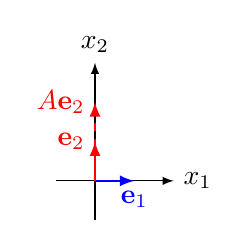
\begin{tikzpicture}[scale=0.5]
		\draw[->] (-1,0) -- (2,0) node[right] {$x_1$};
		\draw[->] (0,-1) -- (0,3) node[above] {$x_2$};
		\draw[thick, blue, ->] (0,0) -- (1,0) node[below] {$\mathbf{e}_1$};
		\draw[thick, red, ->] (0,0) -- (0,1) node[left] {$\mathbf{e}_2$};
		\draw[thick, red, dashed, ->] (0,0) -- (0,2) node[left] {$A\mathbf{e}_2$};
	\end{tikzpicture}
}

\ex{
	\(A = \begin{pmatrix} -1 & 0 \\[6pt] 0 & 1 \end{pmatrix}\)
}{
	\textbf{Transformation:} Reflection about the vertical axis.
	\centering
	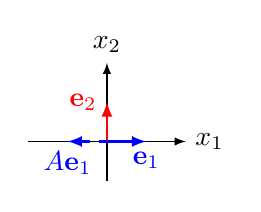
\begin{tikzpicture}[scale=0.5]
		\draw[->] (-2,0) -- (2,0) node[right] {$x_1$};
		\draw[->] (0,-1) -- (0,2) node[above] {$x_2$};
		\draw[thick, blue, ->] (0,0) -- (1,0) node[below] {$\mathbf{e}_1$};
		\draw[thick, red, ->] (0,0) -- (0,1) node[left] {$\mathbf{e}_2$};
		\draw[thick, blue, dashed, ->] (0,0) -- (-1,0) node[below] {$A\mathbf{e}_1$};
	\end{tikzpicture}
}

\ex{
	\(A = \begin{pmatrix} 0 & 1 \\[6pt] 1 & 0 \end{pmatrix}\)
}{
	\textbf{Transformation:} Reflection about the line \(x_1 = x_2\).
	\centering
	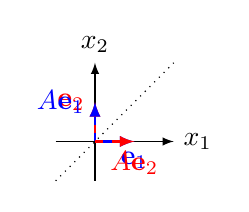
\begin{tikzpicture}[scale=0.5]
		\draw[->] (-1,0) -- (2,0) node[right] {$x_1$};
		\draw[->] (0,-1) -- (0,2) node[above] {$x_2$};
		\draw[thick, blue, ->] (0,0) -- (1,0) node[below] {$\mathbf{e}_1$};
		\draw[thick, red, ->] (0,0) -- (0,1) node[left] {$\mathbf{e}_2$};
		\draw[thick, blue, dashed, ->] (0,0) -- (0,1) node[left] {$A\mathbf{e}_1$};
		\draw[thick, red, dashed, ->] (0,0) -- (1,0) node[below] {$A\mathbf{e}_2$};
		\draw[dotted] (-1,-1) -- (2,2);
	\end{tikzpicture}
}

\ex{
	\(A = \begin{pmatrix}
		\cos\theta & -\sin\theta \\[6pt]
		\sin\theta & \cos\theta
	\end{pmatrix}\)
}{
	\textbf{Transformation:} Counterclockwise rotation by \(\theta\) about the origin.
	\centering
	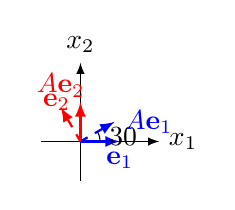
\begin{tikzpicture}[scale=0.5]
		\draw[->] (-1,0) -- (2,0) node[right] {$x_1$};
		\draw[->] (0,-1) -- (0,2) node[above] {$x_2$};
		\def\theta{30}
		\draw[thick, blue, ->] (0,0) -- (1,0) node[below] {$\mathbf{e}_1$};
		\draw[thick, red, ->] (0,0) -- (0,1) node[left] {$\mathbf{e}_2$};
		\draw[thick, blue, dashed, ->] (0,0) -- ({cos(\theta)}, {sin(\theta)}) node[right] {$A\mathbf{e}_1$};
		\draw[thick, red, dashed, ->] (0,0) -- ({-sin(\theta)}, {cos(\theta)}) node[above] {$A\mathbf{e}_2$};
		\draw (0.5,0) arc (0:\theta:0.5) node[midway, right] {$\theta$};
	\end{tikzpicture}
}

\ex{
	\(A = \begin{pmatrix} 0 & 0 \\[6pt] 0 & 1 \end{pmatrix}\)
}{
	\textbf{Transformation:} Projection onto the vertical axis.
	\centering
	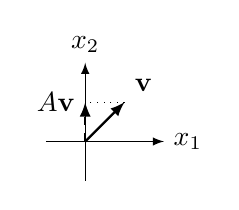
\begin{tikzpicture}[scale=0.5]
		\draw[->] (-1,0) -- (2,0) node[right] {$x_1$};
		\draw[->] (0,-1) -- (0,2) node[above] {$x_2$};
		\draw[thick, ->] (0,0) -- (1,1) node[above right] {$\mathbf{v}$};
		\draw[thick, dashed, ->] (0,0) -- (0,1) node[left] {$A\mathbf{v}$};
		\draw[dotted] (1,1) -- (0,1);
	\end{tikzpicture}
}

\section{Mapping}

\[
	[x_1,\; x_2] \;\longmapsto\; \text{point }(x_1, x_2).
\]

Under the linear transformation given by
\[
	[x_1,\; x_2] \;\mapsto\;
	\begin{bmatrix}
		x_1 + 2x_2 \\
		x_2
	\end{bmatrix},
\]
we see that points are ``stretched to the right'' in the \(x_1\)-direction, while the \(x_2\) coordinate remains unchanged.

\subsection*{Method 1 -- Vector Method}

The matrix under consideration is
\[
	A \;=\; \begin{bmatrix} 1 & 2 \\ 0 & 1 \end{bmatrix}.
\]
The columns of this matrix are:
\[
	\begin{bmatrix} 1 \\ 0 \end{bmatrix}
	\quad\text{and}\quad
	\begin{bmatrix} 2 \\ 1 \end{bmatrix}.
\]
These are the images of the standard basis vectors \(\mathbf{e}_1\) and \(\mathbf{e}_2\), respectively.

\begin{center}
	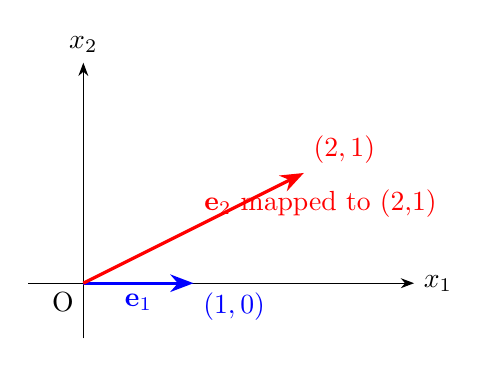
\begin{tikzpicture}[scale=1.4, >=Stealth, baseline={(0,0)}]
		% Axes
		\draw[->] (-0.5,0) -- (3,0) node[right] {\(x_1\)};
		\draw[->] (0,-0.5) -- (0,2) node[above] {\(x_2\)};

		% e1 vector
		\draw[->, very thick, blue] (0,0) -- (1,0) node[midway, below] {\(\mathbf{e}_1\)};

		% e2 vector
		\draw[->, very thick, red] (0,0) -- (2,1) node[midway, above right] {\(\mathbf{e}_2\) mapped to (2,1)};

		% Labels
		\node at (1,0) [below right, blue] {$(1,0)$};
		\node at (2,1) [above right, red] {$(2,1)$};

		\draw (0,0) node[below left] {O};
	\end{tikzpicture}
\end{center}

\subsection*{Method 2 -- Vertex Method}

Consider the unit square with vertices
\[
	(0,0), \quad (1,0), \quad (1,1), \quad (0,1).
\]
We apply \(A\) to each vertex:

\[
	A \begin{bmatrix} 0 \\ 0 \end{bmatrix}
	= \begin{bmatrix} 0 \\ 0 \end{bmatrix},\quad
	A \begin{bmatrix} 1 \\ 0 \end{bmatrix}
	= \begin{bmatrix} 1 \\ 0 \end{bmatrix},\quad
	A \begin{bmatrix} 0 \\ 1 \end{bmatrix}
	= \begin{bmatrix} 2 \\ 1 \end{bmatrix},\quad
	A \begin{bmatrix} 1 \\ 1 \end{bmatrix}
	= \begin{bmatrix} 3 \\ 1 \end{bmatrix}.
\]

Hence the new vertices are \((0,0)\), \((1,0)\), \((2,1)\), and \((3,1)\). Plotting these points yields the transformed parallelogram (the image of the original unit square).

\begin{center}
	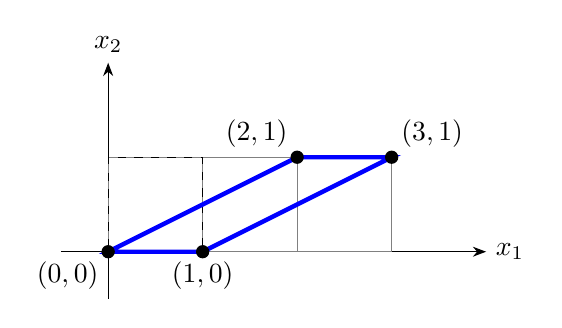
\begin{tikzpicture}[scale=1.2, >=Stealth, baseline={(0,0)}]
		% Axes
		\draw[->] (-0.5,0) -- (4,0) node[right] {\(x_1\)};
		\draw[->] (0,-0.5) -- (0,2) node[above] {\(x_2\)};

		% Original square
		\draw[very thin, gray] (0,0) grid (3,1);

		% Original square edges (dashed)
		\draw[dashed] (0,0) -- (1,0) -- (1,1) -- (0,1) -- cycle;

		% Transformed parallelogram
		\draw[ultra thick, blue] (0,0) -- (1,0) -- (3,1) -- (2,1) -- cycle;

		% Points (labels)
		\fill (0,0) circle (2pt) node[below left] {$(0,0)$};
		\fill (1,0) circle (2pt) node[below] {$(1,0)$};
		\fill (2,1) circle (2pt) node[above left] {$(2,1)$};
		\fill (3,1) circle (2pt) node[above right] {$(3,1)$};
	\end{tikzpicture}
\end{center}

\dfn{Rules for Linear Transformations}{

	\begin{enumerate}
		\item \textbf{Straight lines remain straight.}
		\item \textbf{Parallel lines remain parallel.}
		\item \textbf{Distances along lines scale in a consistent, proportional way.}
	\end{enumerate}
}

\subsubsection{Justification}

\paragraph{1. Straight lines stay straight.}
A line in parametric form is:
\[
	r(t) = t\,\mathbf{v} + \mathbf{w}.
\]
Applying \(A\) gives:
\[
	A(r(t)) = A(t\,\mathbf{v} + \mathbf{w}) = t\,A(\mathbf{v}) + A(\mathbf{w}),
\]
which is again a parametric line.

\paragraph{2. Parallel lines stay parallel.}
If two lines are parallel, their direction vectors are scalar multiples of each other. After applying \(A\), the resulting direction vectors are \(A(\mathbf{v})\) for each original direction \(\mathbf{v}\). Since \(A\) is linear, any scalar multiples remain so, preserving parallelism.

\paragraph{3. Distances scale proportionally.}
For two points \(\mathbf{v}_1\) and \(\mathbf{v}_2\), the difference is \(\mathbf{d} = \mathbf{v}_2 - \mathbf{v}_1\). Under \(A\):
\[
	A\mathbf{v}_2 - A\mathbf{v}_1 = A(\mathbf{v}_2 - \mathbf{v}_1) = A(\mathbf{d}).
\]
Thus the new distance \(\|\mathbf{d}'\| = \|A(\mathbf{d})\|\) is a consistent transform of \(\|\mathbf{d}\|\), depending on the nature of \(A\).

\ex{
	A matrix \(A\) that acts on a parallelogram (spanned by two vectors \(\mathbf{x}_1, \mathbf{x}_2\)) will produce another parallelogram in the output plane.
}{
	\begin{center}
		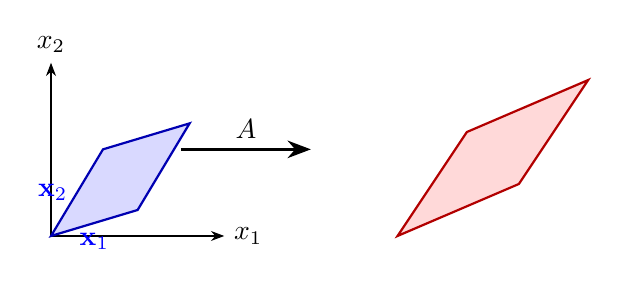
\begin{tikzpicture}[scale=1.1, >=Stealth, baseline={(0,0)}]
			% Original parallelogram
			\coordinate (O) at (0,0);
			\coordinate (X1) at (1,0.3);
			\coordinate (X2) at (0.6,1);

			\draw[->] (O) -- ++(2,0) node[right] {\(x_1\)};
			\draw[->] (O) -- ++(0,2) node[above] {\(x_2\)};

			\filldraw[fill=blue!15, draw=blue!70!black, thick]
			(O) -- (X1) -- ($(X1)+(X2)$) -- (X2) -- cycle;
			\node at ($(X1)!0.5!(O)$) [below, blue] {\(\mathbf{x}_1\)};
			\node at ($(X2)!0.5!(O)$) [left, blue] {\(\mathbf{x}_2\)};

			% Arrow indicating transformation
			\draw[->, very thick] (1.5,1) -- (3,1) node[midway, above] {$A$};

			% Transformed parallelogram
			% Let's define some coordinates for the transformed shape
			\coordinate (O2) at (4,0);               % Shift for the second shape
			\coordinate (X1t) at ($(O2)+(1.4,0.6)$); % Some transformed version of x1
			\coordinate (X2t) at ($(O2)+(0.8,1.2)$); % Some transformed version of x2

			\filldraw[fill=red!15, draw=red!70!black, thick]
			(O2) -- (X1t) -- ($(X1t)+(X2t)-(O2)$) -- (X2t) -- cycle;
		\end{tikzpicture}
	\end{center}

	\noindent
	\emph{Here, lines remain lines, parallels remain parallel.}
}

\section{A System of Linear Equations}

We have a matrix \(A\) of size \(m \times n\), multiplying an unknown vector
\(\begin{bmatrix} x_1 \\ x_2 \\ \vdots \\ x_n \end{bmatrix}\)
(which belongs to \(\mathbb{R}^n\)), producing a result vector
\(\begin{bmatrix} v_1 \\ v_2 \\ \vdots \\ v_m \end{bmatrix}\)
in \(\mathbb{R}^m\):
\[
	A_{m \times n}
	\begin{bmatrix}
		x_1    \\
		x_2    \\
		\vdots \\
		x_n
	\end{bmatrix}
	=
	\begin{bmatrix}
		v_1    \\
		v_2    \\
		\vdots \\
		v_m
	\end{bmatrix}.
\]

This can be viewed as a \emph{system of \(m\) linear equations in \(n\) unknowns}. We are often interested in two main questions:

\begin{enumerate}
	\item \textbf{Does a solution exist?}
	      That is, can we find \(x_1, x_2, \dots, x_n\) so that \(A\mathbf{x} = \mathbf{v}\)?
	      Geometrically, this asks if \(\mathbf{v}\) lies in the \emph{column space} (or image) of \(A\).

	\item \textbf{If at least one solution exists, is it unique or are there infinitely many?}
	      Uniqueness is typically tied to whether the columns of \(A\) are linearly independent (and whether \(m\), \(n\) are related in a way that gives a single solution).  If there are \emph{fewer} pivots than unknowns, or if the system is underdetermined, infinitely many solutions can occur.
\end{enumerate}

\vspace{1em}
\noindent
\textit{Key intuition:}
\begin{itemize}
	\item The question of \emph{existence} boils down to whether \(\mathbf{v}\) is in the span of the columns of \(A\).
	\item The question of \emph{uniqueness} depends on whether those columns form a set of independent vectors and on the relationship between \(m\) and \(n\).
\end{itemize}


\section{How to Determine Consistency, Uniqueness, and the Number of Solutions for a Linear System}
\nt{
	We consider a linear system
	\[
		\begin{cases}
			a_{11} x_1 \;+\; a_{12} x_2 \;+\; \cdots + a_{1n} x_n \;=\; b_1 \\[6pt]
			a_{21} x_1 \;+\; a_{22} x_2 \;+\; \cdots + a_{2n} x_n \;=\; b_2 \\
			\vdots &                                                        \\
			a_{m1} x_1 \;+\; a_{m2} x_2 \;+\; \cdots + a_{mn} x_n \;=\; b_m
		\end{cases}
	\]
	and write it in \emph{augmented matrix} form:
	\[
		\bigl[A \mid \mathbf{b}\bigr]
		\;=\;
		\begin{bmatrix}
			a_{11} & a_{12} & \cdots & a_{1n} & b_1    \\
			a_{21} & a_{22} & \cdots & a_{2n} & b_2    \\
			\vdots & \vdots & \ddots & \vdots & \vdots \\
			a_{m1} & a_{m2} & \cdots & a_{mn} & b_m
		\end{bmatrix}.
	\]

	\begin{itemize}
		\item We perform \emph{elementary row operations} (EROs) on \(\bigl[A \mid \mathbf{b}\bigr]\) to attempt to solve the system. The EROs are:
		      \begin{enumerate}
			      \item \textbf{Scaling (multiplying a row by a nonzero constant).}
			      \item \textbf{Row replacement} (\(R_i \;=\; R_i \;+\; c\,R_j\) for \(i\neq j\)).
			      \item \textbf{Interchanging two rows} (\(R_i \leftrightarrow R_j\)).
		      \end{enumerate}
		      These operations do not change the solution set of the system.
	\end{itemize}

	\textbf{Row Echelon Form (REF)}
	We say \(\bigl[A\mid\mathbf{b}\bigr]\) is in \emph{row echelon form} if:
	\begin{itemize}
		\item All rows of all zeros (if any) are at the bottom of the matrix.
		\item Each \emph{pivot} (leftmost nonzero entry in a nonzero row) is strictly to the right of the pivot in the row above.
	\end{itemize}
	A pivot column in \(A\) corresponds to a \emph{leading variable} (or \emph{basic variable}), and any other column (apart from the augmented column) is called a \emph{free column} (its corresponding variable is a \emph{free variable}).

	\textbf{Consistency \& Number of Solutions}
	\begin{itemize}
		\item If, in the augmented matrix, there is a pivot in the last column (meaning a row of the form
		      \[
			      [\,0\quad 0\quad \cdots\quad 0 \mid c\,],\quad c \neq 0,
		      \]
		      ) then the system is \emph{inconsistent} (no solutions). This corresponds to an equation \(0 = c\) where \(c\neq 0\), which is impossible.
		\item If no such contradiction is found, then at least one solution exists (the system is \emph{consistent}).
		\item The number of pivot columns in \(A\) (i.e.\ the number of leading variables) tells us whether solutions are unique or infinite:
		      \begin{enumerate}
			      \item If the number of pivots equals the number of unknowns \(n\), then there is exactly one solution (assuming no inconsistency).
			      \item If the number of pivots is less than \(n\), then there are free variables, implying infinitely many solutions (again, assuming no inconsistency).
		      \end{enumerate}
	\end{itemize}

	\ex{Example: Augmented Matrix and REF}{
		\[
			\begin{bmatrix}
				1 & 2 & 3 & 5  \\
				2 & 4 & 6 & 9  \\
				3 & 6 & 9 & 15
			\end{bmatrix}
			\;\longrightarrow\;\text{(REF)}.
		\]
		One performs row operations to get an upper-triangular or echelon form.  If the last row becomes something like
		\[
			[\,0\;\;0\;\;0\mid c\,], \quad c\neq 0,
		\]
		then there is no solution.  Otherwise, we identify pivot columns, read off the relationships among variables, and find a general solution (unique or infinite).
	}

	\dfn{Free Columns and Basic Columns}{
		Once an augmented matrix is in REF, we label each pivot column (in \(A\)) as a \emph{basic column}, and any other column (except the last augmented column) as a \emph{free column}.
		\begin{itemize}
			\item If \(x_j\) corresponds to a free column, we may label \(x_j\) as a parameter (e.g.\ \(t_1, t_2, \dots\)).
			\item The variables in pivot columns can then be written in terms of these parameters.
		\end{itemize}
		In this manner, we get a general solution describing the entire solution set to \(A\mathbf{x} = \mathbf{b}\).
	}

	\textbf{Algorithm to Convert \(\bigl[A\mid \mathbf{b}\bigr]\) to \(\mathrm{REF}(A)\)}
	\begin{enumerate}
		\item \emph{Select a candidate row}: Choose the topmost row \emph{among those not yet having a pivot} in which a pivot might appear.
		\item \emph{Pivot search and possible row swap}: Among this candidate row and those below it, find a row having a leftmost nonzero entry in the desired pivot column. Interchange (swap) that row with the candidate row if needed, placing a nonzero entry where your pivot should be.
		\item \emph{Declare the pivot and eliminate below}: Scale the pivot row (if desired) so that the pivot becomes \(1\). Then use row replacement to produce zeros below that pivot in the same column.
		\item Move to the next row down and next column to the right, and repeat until you have a row echelon form.
	\end{enumerate}

	One can then further use row replacement operations to clear the entries \emph{above} each pivot, yielding the \emph{reduced} row echelon form (RREF). However, for most solution purposes, REF is already sufficient to read off whether solutions exist, how many, and so on.
}
\subsection{FRR}
\begin{algorithm}[H]
	\KwIn{Matrix \(A\) of size \(m \times n\) and vector \(\mathbf{b}\) of size \(m\)}
	\KwOut{Upper triangular matrix \(A\) and modified vector \(\mathbf{b}\)}
	\SetAlgoLined
	\SetNoFillComment
	\tcc{Forward elimination process}
	\For{$k \leftarrow 1$ \KwTo $\min(m, n)$}{
		\For{$i \leftarrow k+1$ \KwTo $m$}{
			\If{$A_{kk} \neq 0$}{
				$f \leftarrow A_{ik} / A_{kk}$\;
				\For{$j \leftarrow k$ \KwTo $n$}{
					$A_{ij} \leftarrow A_{ij} - f \cdot A_{kj}$\;
				}
				$b_i \leftarrow b_i - f \cdot b_k$\;
			}
		}
	}
	\Return $A, \mathbf{b}$\;
	\caption{Forward Row Reduction (Forward Elimination)}
\end{algorithm}

\section{Back Row Reduction}

\nt{
	Back row reduction, also known as back substitution, is a method used to solve a system of linear equations that has been transformed into an upper triangular form through Gaussian elimination. This method involves solving the equations starting from the last row and moving upwards.
}

\dfn{Back Row Reduction}{
	Consider a system of linear equations represented in matrix form as \(A\mathbf{x} = \mathbf{b}\), where \(A\) is an upper triangular matrix:
	\[
		\begin{bmatrix}
			a_{11} & a_{12} & \cdots & a_{1n} \\
			0      & a_{22} & \cdots & a_{2n} \\
			\vdots & \vdots & \ddots & \vdots \\
			0      & 0      & \cdots & a_{nn}
		\end{bmatrix}
		\begin{bmatrix}
			x_1    \\
			x_2    \\
			\vdots \\
			x_n
		\end{bmatrix}
		=
		\begin{bmatrix}
			b_1    \\
			b_2    \\
			\vdots \\
			b_n
		\end{bmatrix}.
	\]
	The solution is obtained by solving the last equation first and then substituting the obtained values into the preceding equations.
}

\ex{Example of Back Row Reduction}{
	Consider the following upper triangular system:
	\[
		\begin{cases}
			2x_1 + 3x_2 + 4x_3 = 5, \\
			0x_1 + 6x_2 + 7x_3 = 8, \\
			0x_1 + 0x_2 + 9x_3 = 10.
		\end{cases}
	\]
	We start with the last equation:
	\[
		9x_3 = 10 \quad \Rightarrow \quad x_3 = \frac{10}{9}.
	\]
	Next, we substitute \(x_3\) into the second equation:
	\[
		6x_2 + 7\left(\frac{10}{9}\right) = 8 \quad \Rightarrow \quad 6x_2 + \frac{70}{9} = 8 \quad \Rightarrow \quad 6x_2 = 8 - \frac{70}{9} \quad \Rightarrow \quad x_2 = \frac{2}{9}.
	\]
	Finally, we substitute \(x_2\) and \(x_3\) into the first equation:
	\[
		2x_1 + 3\left(\frac{2}{9}\right) + 4\left(\frac{10}{9}\right) = 5 \quad \Rightarrow \quad 2x_1 + \frac{6}{9} + \frac{40}{9} = 5 \quad \Rightarrow \quad 2x_1 = 5 - \frac{46}{9} \quad \Rightarrow \quad x_1 = \frac{1}{9}.
	\]
	Thus, the solution is:
	\[
		x_1 = \frac{1}{9}, \quad x_2 = \frac{2}{9}, \quad x_3 = \frac{10}{9}.
	\]
}

\begin{algorithm}[H]
	\KwIn{Upper triangular matrix \(A\) of size \(n \times n\) and vector \(\mathbf{b}\) of size \(n\)}
	\KwOut{Solution vector \(\mathbf{x}\) of size \(n\)}
	\SetAlgoLined
	\SetNoFillComment
	\tcc{Initialize solution vector}
	\For{$i \leftarrow n$ \KwTo $1$}{
		$x_i \leftarrow b_i$\;
		\For{$j \leftarrow i+1$ \KwTo $n$}{
			$x_i \leftarrow x_i - A_{ij} \cdot x_j$\;
		}
		$x_i \leftarrow x_i / A_{ii}$\;
	}
	\Return $\mathbf{x}$\;
	\caption{Back Row Reduction (Back Substitution)}
\end{algorithm}

\ex{Full SLE solving}{
	$$ \begin{bmatrix}
			1 & 1  & 2 & 2  \\
			1 & -1 & 0 & -2 \\
			2 & 0  & m & 0
		\end{bmatrix}
	$$
	$$
		\begin{bmatrix}
			1 & 1  & 2   & 2  \\
			0 & -2 & -2  & -4 \\
			0 & -2 & m-4 & -4
		\end{bmatrix}
	$$
	$$
		\begin{bmatrix}
			1 & 1  & 2   & 2  \\
			0 & -2 & -2  & -4 \\
			0 & 0  & m-2 & 0
		\end{bmatrix}
	$$
	given m=0
	$$
		\begin{bmatrix}
			1 & 1  & 2  & 2  \\
			0 & -2 & -2 & -4 \\
			0 & 0  & 0  & 0
		\end{bmatrix}
	$$
	$$
		\begin{bmatrix}
			1 & 1 & 2 & 2 \\
			0 & 1 & 1 & 2 \\
			0 & 0 & 0 & 0
		\end{bmatrix}
	$$
	$$
		\begin{bmatrix}
			1 & 0 & 1 & 0 \\
			0 & 1 & 1 & 2 \\
			0 & 0 & 0 & 0
		\end{bmatrix}
	$$

}

\chapter{Linear Combinations}



\section{Matrix--Vector Product as Linear Combination}

\[
	\begin{aligned}
		A x
		 & =
		\begin{bmatrix}
			1 & -2  \\[6pt]
			3 & \;2
		\end{bmatrix}
		\begin{bmatrix}
			x_1 \\[3pt]
			x_2
		\end{bmatrix}
		= x_1
		\begin{bmatrix} 1 \\[3pt] 3 \end{bmatrix}
		+ x_2
		\begin{bmatrix} -2 \\[3pt] 2 \end{bmatrix}
		= b.
	\end{aligned}
\]

\textit{Intuition:} ``Scaling each column of \(A\) by its corresponding entry in \(x\).''

In other words, to compute \(A x\), you take \(x_1\) times the first column of \(A\) plus \(x_2\) times the second column of \(A\).


\ex{ A Specific Choice of \(x\)}{
	If
	\[
		A =
		\begin{bmatrix}
			1 & -2    \\[3pt]
			3 & \;\,2
		\end{bmatrix},
	\]
	then the first column is
	\[
		a_1 = \begin{bmatrix} 1 \\ 3 \end{bmatrix}
		\quad\text{and}\quad
		a_2 = \begin{bmatrix} -2 \\ 2 \end{bmatrix}.
	\]
	A linear combination of these columns is
	\[
		x_1 \begin{bmatrix} 1 \\ 3 \end{bmatrix}
		\;+\;
		x_2 \begin{bmatrix} -2 \\ 2 \end{bmatrix}
		\;=\;
		b.
	\]

	As an example, if \(x_1 = -\tfrac{1}{3}\) and \(x_2 = 1\),
	\[
		-\tfrac{1}{3}
		\begin{bmatrix} 1 \\ 3 \end{bmatrix}
		\;+\;
		\begin{bmatrix} -2 \\ 2 \end{bmatrix}
		=
		\begin{bmatrix}
			-\tfrac{1}{3} - 2 \\[4pt]
			-1 + 2
		\end{bmatrix}
		=
		\begin{bmatrix}
			-\tfrac{7}{3} \\[4pt]
			1
		\end{bmatrix}.
	\]
	In the notes, a similar combination yields \(\begin{bmatrix}-2 \\ -2\end{bmatrix}\). The key point is that any pair \((x_1,x_2)\) gives a vector in \(\mathbb{R}^2\).
}

\dfn{Span}{
	\textbf{Span} of a set of vectors is the collection of all linear combinations of those vectors. Concretely, for
	\[
		a_1 = \begin{bmatrix} 1 \\ 3 \end{bmatrix},
		\quad
		a_2 = \begin{bmatrix} -2 \\ 2 \end{bmatrix},
	\]
	we write
	\[
		\mathrm{Span}\{\,a_1, a_2\}
		=\Bigl\{\,
		x_1 a_1 + x_2 a_2
		\;\big|\;
		x_1, x_2 \in \mathbb{R}
		\Bigr\}.
	\]
	Any vector \(b\) not in this span means \(A x = b\) has no solution.
}

\section{Linear Combinations and the Span}
Vectors ``outside'' the span of \(\{a_1,a_2\}\) are precisely those \(b\) for which the system \(A x = b\) is not consistent. Equivalently, they are not expressible as a linear combination of \(a_1\) and \(a_2\).


\section{Geometric Plots in the Notes}

\begin{enumerate}
	\item \textit{First Plot (showing the columns \(a_1\) and \(a_2\)):}

	      \begin{center}
		      \begin{tikzpicture}[scale=0.8,>=stealth]
			      % axes
			      \draw[->] (-0.5,0) -- (3.5,0) node[right] {\(x\)};
			      \draw[->] (0,-0.5) -- (0,3.5) node[above] {\(y\)};

			      % a_1 vector
			      \draw[->,thick,blue] (0,0) -- (1,3) node[midway,left] {\(\displaystyle a_1\)};

			      % a_2 vector
			      \draw[->,thick,red] (0,0) -- (-2,2) node[midway,above] {\(\displaystyle a_2\)};

			      % a rough parallelogram to illustrate a typical combination
			      \draw[dashed] (1,3) -- (1-2,3+2);
			      \draw[dashed] (-2,2) -- (-2+1,2+3);
		      \end{tikzpicture}
	      \end{center}

	      Any linear combination \(x_1 a_1 + x_2 a_2\) lands in the parallelogram structure (and its extensions) formed by these two vectors.

	\item \textit{Second Plot (showing a vector not in the span)}:

	      \begin{center}
		      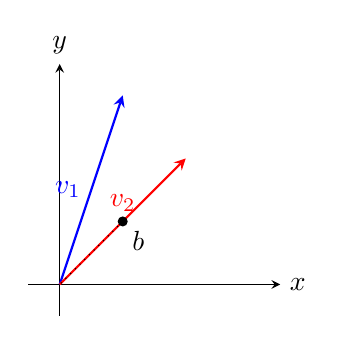
\begin{tikzpicture}[scale=0.8,>=stealth]
			      % axes
			      \draw[->] (-0.5,0) -- (3.5,0) node[right] {\(x\)};
			      \draw[->] (0,-0.5) -- (0,3.5) node[above] {\(y\)};

			      % example vectors v1, v2 (suppose they are the same as above or placeholders)
			      \draw[->,thick,blue] (0,0) -- (1,3) node[midway,left] {\(\displaystyle v_1\)};
			      \draw[->,thick,red] (0,0) -- (2,2) node[midway,above] {\(\displaystyle v_2\)};

			      % a point b that is not in the span
			      \filldraw[black] (1,1) circle (2pt) node[below right] {\(\displaystyle b\)};

			      % dashed lines to illustrate that b is not on the plane spanned by v1 and v2
			      % (just a conceptual marker)
			      \draw[dotted] (1,1) -- (0,0);
		      \end{tikzpicture}
	      \end{center}

	      If \(v_1\) and \(v_2\) do not cover \((1,1)\) by any linear combination, then \(\begin{bmatrix}1\\1\end{bmatrix}\) is not in their span, hence no solution exists for \(Ax=b\).

	\item \textit{Plot illustrating parallel vectors}:

	      \begin{center}
		      \begin{tikzpicture}[scale=0.8,>=stealth]
			      % axes
			      \draw[->] (-0.5,0) -- (4,0) node[right] {\(x\)};
			      \draw[->] (0,-0.5) -- (0,4) node[above] {\(y\)};

			      % two parallel vectors
			      \draw[->,thick,blue] (0,0) -- (2,2) node[midway,above left] {\(\displaystyle v_1\)};
			      \draw[->,thick,blue!50!green] (0,0) -- (3,3) node[midway,above] {\(\displaystyle v_2\)};

			      % a vector b not on that line
			      \filldraw[red] (2,3) circle (2pt) node[right] {\(\displaystyle b\)};

			      % line indication
			      \draw[dashed] (0,0) -- (3.5,3.5);
		      \end{tikzpicture}
	      \end{center}

	      Here, \(v_1\) and \(v_2\) are multiples of each other, so their span is just the single dashed line. The vector \(b\) off that line cannot be written as any combination of \(v_1\) and \(v_2\).
\end{enumerate}

\ex{$\vec{b}$ not in span of $\vec{v_1}, \vec{v_2}$}{
	\tdplotsetmaincoords{70}{110}
	\centering
	\begin{tikzpicture}[tdplot_main_coords, scale=2]
		% Draw coordinate axes
		\draw[->, thick] (0,0,0) -- (2,0,0) node[anchor=north east] {$x$};
		\draw[->, thick] (0,0,0) -- (0,2,0) node[anchor=north west] {$y$};
		\draw[->, thick] (0,0,0) -- (0,0,2) node[anchor=south] {$z$};

		% Draw the plane spanned by v1 and v2.
		% Every vector in the span has x = y, so we fill the plane { (u,u,w) : u,w in R }.
		% Here we choose a rectangular patch with u from -1 to 1 and w from -1 to 2.
		\filldraw[fill=blue!20, draw=blue, opacity=0.5]
		(-1,-1,-1) -- (1,1,-1) -- (1,1,2) -- (-1,-1,2) -- cycle;

		% Draw vector v1 = (1,1,1)
		\draw[-{Stealth[scale=1.2]}, red, thick] (0,0,0) -- (1,1,1)
		node[midway, anchor=south east] {$v_1$};

		% Draw vector v2 = (-1,-1,1)
		\draw[-{Stealth[scale=1.2]}, red, thick] (0,0,0) -- (-1,-1,1)
		node[midway, anchor=north west] {$v_2$};

		% Draw vector b = (1,0,0)
		\draw[-{Stealth[scale=1.2]}, green!70!black, thick] (0,0,0) -- (1,0,0)
		node[midway, anchor=south] {$b$};

		% Add an annotation that b is not in the span of v1 and v2.
		\node at (2.5, 2, 0.5) {$b\notin\operatorname{span}\{v_1,v_2\}$};
	\end{tikzpicture}
}

\subsection{Key Conclusions}

\begin{itemize}
	\item \(\mathrm{Span}\{a_1, a_2\}\) is the set of all vectors \(b\) for which \(Ax = b\) has a solution.
	\item If \(b\) is not in that span, there is no solution.
	\item Geometrically, if \(a_1\) and \(a_2\) are not multiples of each other, their span is a 2D plane through the origin in \(\mathbb{R}^2\). If they are multiples, the span is just a single line, and most vectors in \(\mathbb{R}^2\) lie outside that line (no solution).
	\item $span{a_1}$ is a line or point. $span{a_1, a_2}$ is a plane, line or point. and so on
\end{itemize}

\subsection{Dropping a vector to retain the same span}

\qs{Drop vector $a_3$ to retain the same span as $a_1$, $a_2$ and $a_3$.}{
	\[
		a_1 =
		\begin{bmatrix}
			2 \\ 1
		\end{bmatrix}
	\]

	\[
		a_2 =
		\begin{bmatrix}
			1 \\ 1
		\end{bmatrix}
	\]

	\[
		a_3 =
		\begin{bmatrix}
			3 \\ 3
		\end{bmatrix}
	\]
}

\sol
yes, $span{a_1,a_2,a_3}=span{a_1,a_2}$ because $a_3$ is a linear combination of $a_1$ and $a_2$ ($a_1+a_2a_3$)

\section{Evaluating Linear Dependence Procedurally}

\ex{
	Finding linear dependence of a set of vectors.
}{
	\[
		\vec{v_1} =
		\begin{bmatrix}
			1 \\2\\3
		\end{bmatrix}
		,
		\vec{v_2} =
		\begin{bmatrix}
			3 \\2\\1
		\end{bmatrix}
		,
		\vec{v_3} =
		\begin{bmatrix}
			5 \\2\\-1
		\end{bmatrix}
	\]
	Since $v_3$ is a linear combination of $v_1$ and $v_2$, we can drop $v_3$ to retain the same span as $v_1$ and $v_2$.
	\[
		span{v_1,v_2,v_3} = span{v_1,v_2}
	\]
	As
	\[
		v_3 = 2v_1 - v_2
	\]
}

\nt{Working towards a procedure for evaluating linear dependence of a set of vectors.}

\[
	-v_1 + 2v_2 -v_3 = 0
\]

\[
	\begin{bmatrix}
		\vec{v_1} & \vec{v_2} & \vec{v_3}
	\end{bmatrix}
	\begin{bmatrix}
		x_1 \\ x_2 \\ x_3
	\end{bmatrix}
	=
	\begin{bmatrix}
		0 \\ 0 \\ 0
	\end{bmatrix}
\]

We know that one solution is

\[
	\begin{bmatrix}
		x_1 \\ x_2 \\ x_3
	\end{bmatrix}
	=
	\begin{bmatrix}
		-1 \\2\\-1
	\end{bmatrix}
\]

Since this SLE has one particular solution as well as the trivial one, then it must have infinitely many solutions.\\
Then if \(A \vec{x} = 0\) has infinitely many solutions, then the set of vectors (columns) in \(A\) is linearly dependent.\\
Conversely, if \(A \vec{x} = 0\) has only one solution $(\vec{x} = \vec{0})$, then the set of vectors (columns) in \(A\) is linearly independent.\\

\dfn{Linear Independence}{
	We say a set of vectors $\{v_1, v_2, \cdots, v_n\}$ is \emph{linearly independent} if the only solution to the SLE
	\[
		\begin{bmatrix}
			\vec{v_1} & \vec{v_2} & \cdots & \vec{v_n}
		\end{bmatrix}
		\begin{bmatrix}
			x_1 \\ x_2 \\ \vdots \\ x_n
		\end{bmatrix}
		=
		\begin{bmatrix}
			0 \\ 0 \\ \vdots \\ 0
		\end{bmatrix}
	\]
	is the trivial solution, i.e. $\vec{x} = \vec{0}$.\\
}

\[
	A' =
	\begin{bmatrix}
		1 & 3 & 5  & 0 \\
		2 & 2 & 2  & 0 \\
		3 & 1 & -1 & 0
	\end{bmatrix}
	\xrightarrow{R_2 = R_2 - 2R_1, \quad R_3 = R_3 - 3R_1}
	\begin{bmatrix}
		1 & 3  & 5   & 0 \\
		0 & -4 & -8  & 0 \\
		0 & -8 & -16 & 0
	\end{bmatrix}
	\xrightarrow{R_3 = R_3 - 2R_2}
	\begin{bmatrix}
		1 & 3  & 5  & 0 \\
		0 & -4 & -8 & 0 \\
		0 & 0  & 0  & 0
	\end{bmatrix}
	= \text{REF}(A')
\]

1 Free variable $\implies$ Linearly Independent

\[
	\text{REF}(A')
	\xrightarrow{R_2 = R_2 / (-4)}
	\begin{bmatrix}
		1 & 3 & 5 & 0 \\
		0 & 1 & 2 & 0 \\
		0 & 0 & 0 & 0
	\end{bmatrix}
	\xrightarrow{R_1 = R_1 - 3R_2}
	\begin{bmatrix}
		1 & 0 & -1 & 0 \\
		0 & 1 & 2  & 0 \\
		0 & 0 & 0  & 0
	\end{bmatrix}
	= \text{RREF}(A')
	\begin{bmatrix}
		x_1 \\
		x_2 \\
		x_3
	\end{bmatrix}
\]

Then 

\[
	\begin{bmatrix}
		\vec{v_1} & \vec{v_2} & \vec{v_3}
	\end{bmatrix}
	t_3
	\begin{bmatrix}
		1\\-2\\1
	\end{bmatrix}
	= 
	\begin{bmatrix}
		0\\0\\0
	\end{bmatrix}
\]

And therefore the linear combination in its homogeneous form implies

\[
	t_3 (\vec{v_1} - 2\vec{v_2} + \vec{v_3}) = \vec{0}
\]



\end{document}